\documentclass[xcolor=table,bigger,unknownkeysallowed]{beamer}
%\documentclass[unknownkeysallowed]{beamer}
\usepackage[utf8]{inputenc}
\usepackage[T1]{fontenc}
\usepackage[english]{babel}
\usepackage{fixltx2e}
\usepackage{graphicx}
\usepackage{epsfig}
\usepackage{longtable}
\usepackage{float}
\usepackage{wrapfig}
\usepackage{soul}
\usepackage{textcomp}
\usepackage{marvosym}
\usepackage{wasysym}
\usepackage{latexsym}
\usepackage{amssymb}
\usepackage{tabu}
\usepackage{tabularx}
\usepackage{booktabs}
\usepackage[margin=15pt,font={small,sf,it},labelfont=bf]{caption} 
\usepackage{hyperref}
\tolerance=1000
\providecommand{\alert}[1]{\textbf{#1}}
\usepackage{etoolbox}
\newcommand{\icon}[1]{\includegraphics[height=20pt,width=20pt]{#1}}
\usepackage{pgfplots}
\usepackage{tabu}
\usepackage{subcaption}
\usepackage{multirow}


\usepackage{tikz}
\usetikzlibrary{matrix,positioning,fit,fadings}
\def\drowsyColor{green!80!black}       

\title{Out of Hypervisor (OoH)}
\author{Pr Alain Tchana - (alain.tchana@ens-lyon.fr)\\
ENS Lyon}
\date{~}

\usepackage{booktabs}
\usepackage[natbib=true, bibstyle=authoryear, citestyle=authoryear-comp]{biblatex}
\usepackage{beamerthemesplit}
\usetheme{progressbar}
\usecolortheme{progressbar}
\institute{\vskip1ex EuroDW'22 - March, 5}
%\subtitle{subtitle}
\definecolor{tableShade}{HTML}{787878}
\definecolor{tableShade2}{HTML}{606060}
%\setbeamersize{text margin left=.5cm,text margin right=.5cm}
\progressbaroptions{headline=none, frametitle=ckcompliant}
\newcommand{\myitem}{\item[\vspace{0.5ex}]}
\usepackage{lmodern}
\usepackage{ulem} 
\AtBeginSection[]
{
  \begin{frame}<beamer>
    %\frametitle{Outline for section \thesection}
    \tableofcontents[currentsection]
  \end{frame}
}

\setbeamersize{text margin left=0em,text margin right=0em}

\usepackage{tikz,pgfplots}
\usetikzlibrary{pgfplots.groupplots}
\usepackage{pgfplotstable}
\usepgfplotslibrary{external} 
\usetikzlibrary{patterns}
\usepgfplotslibrary{fillbetween}
\usetikzlibrary{matrix,positioning,fit,fadings}
\tikzfading[name=energyPropFading,bottom color=transparent!100,top color=transparent!0]
\usepackage{color, colortbl}
\hypersetup{}

\definecolor{codegreen}{rgb}{0,0.6,0}
\definecolor{codegray}{rgb}{0.5,0.5,0.5}
\definecolor{codepurple}{rgb}{0.58,0,0.82}
\definecolor{backcolour}{rgb}{0.95,0.95,0.92}
\definecolor{americanrose}{rgb}{1.0, 0.01, 0.24}
\definecolor{airforceblue}{rgb}{0.0, 0.0, 1.0}

\newenvironment{variableblock}[3]{%
  \setbeamercolor{block body}{#2}
  \setbeamercolor{block title}{#3}
  \begin{block}{#1}}{\end{block}}

\tikzfading[name=myfading, bottom color=transparent!100, top color=transparent!0]
\begin{document}

\maketitle

%%%%%%%%%%%%%%%%%%%%%%%%%%%%%%%%%%%%%%%%%%%%%%%%%%%%%%%%%%%%%%%%%%%%%%%%%%%%%%%%%%%
        \begin{frame}
        \frametitle{About me} 
			\begin{itemize}
				\item Originate from Cameroon, in Africa
				\item Moved to France for an internship in 2008
				\item 2030, back to Cameroon
				\begin{itemize}
					\item President of the republic: 2032 $\rightarrow \infty$	
\end{itemize}					
			\end{itemize}
 		    \begin{figure}
			\centering
	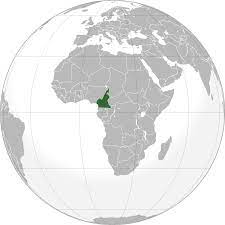
\includegraphics[width=.3\columnwidth]{fig/cameroun.jpeg}
			\end{figure}	
        \end{frame}
%%%%%%%%%%%%%%%%%%%%%%%%%%%%%%%%%%%%%%%%%%%%%%%%%%%%%%%%%%%%%%%%%%%%%%%%%%%%%%%%%%%
        \begin{frame}
        \frametitle{Some famous cameroonians} 
 		    \begin{figure}
			\centering
	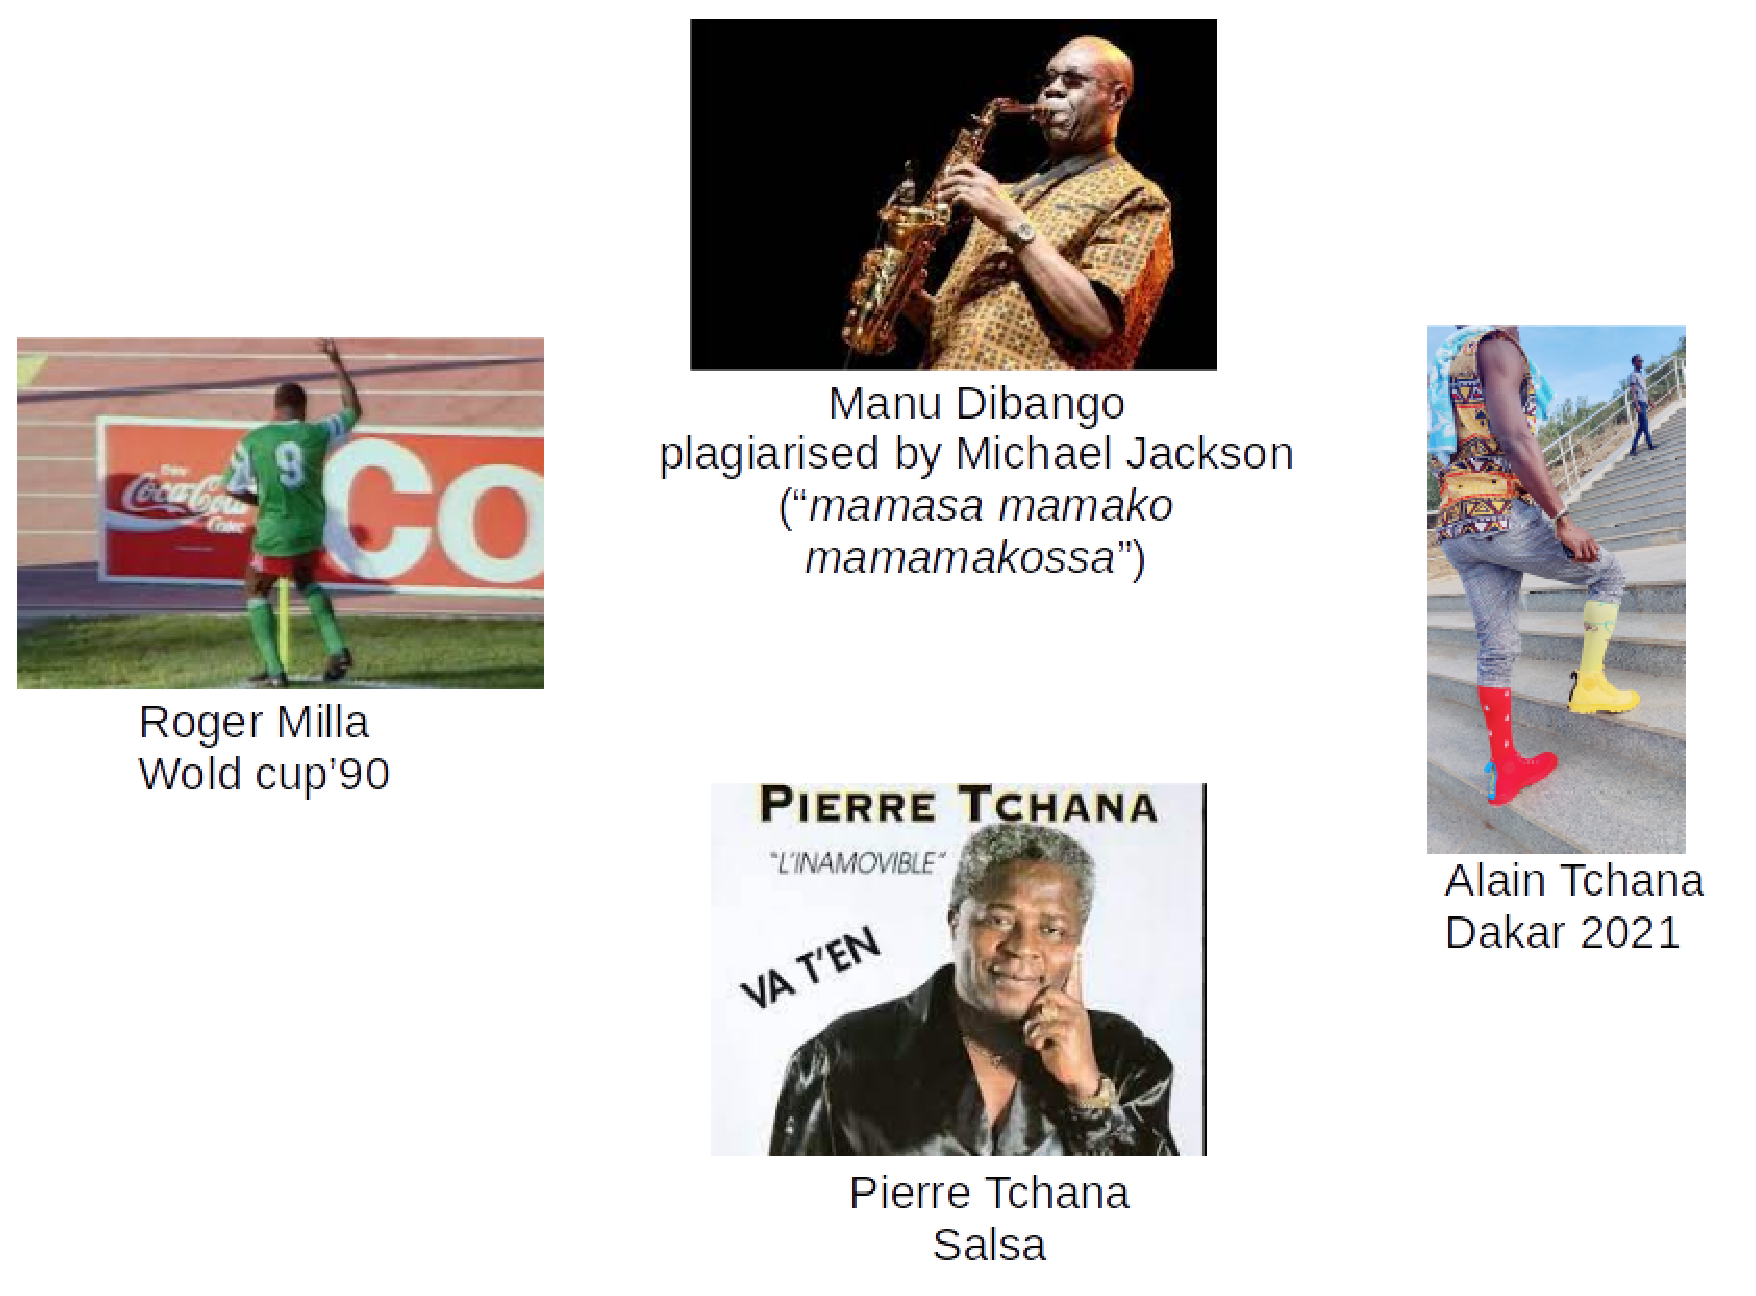
\includegraphics[width=.7\columnwidth]{fig/famous}
			\end{figure}			
        \end{frame}        
%%%%%%%%%%%%%%%%%%%%%%%%%%%%%%%%%%%%%%%%%%%%%%%%%%%%%%%%%%%%%%%%%%%%%%%%%%%%%%%%%%%
        \begin{frame}
        \frametitle{My group} 
			\begin{block}{PhD students}
				\begin{itemize}
					\item 2 females (S. Bitchebe, J. Kouam) and 3 males (K. Nguetchouang, Y. Kone, and T. Dubuc)
				\end{itemize}
			\end{block}
			\begin{block}{Interns}
				\begin{itemize}
					\item 0 female (:() and 3 males (B. Teguia, A. Leberre, R. Colin)
				\end{itemize}
			\end{block}	
 		    \begin{figure}
			\centering
	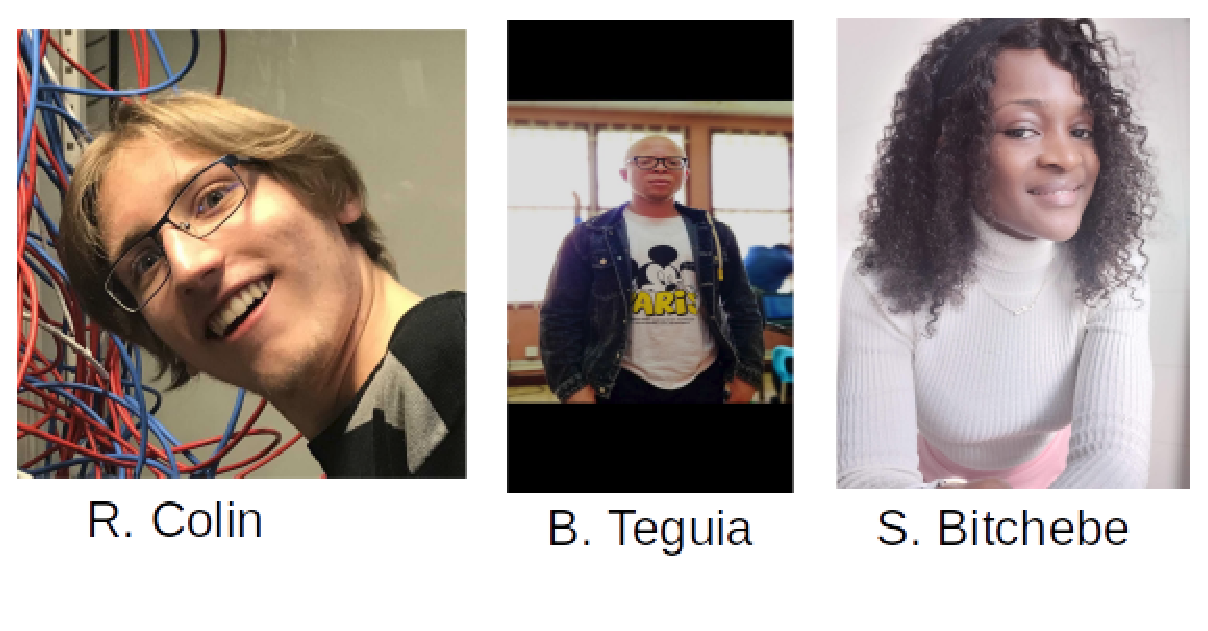
\includegraphics[width=.5\columnwidth]{fig/students}
			\end{figure}						
        \end{frame}
%%%%%%%%%%%%%%%%%%%%%%%%%%%%%%%%%%%%%%%%%%%%%%%%%%%%%%%%%%%%%%%%%%%%%%%%%%%%%%%%%%%
\section{OoH}
%%%%%%%%%%%%%%%%%%%%%%%%%%%%%%%%%%%%%%%%%%%%%%%%%%%%%%%%%%%%%%%%%%%%%%%%%%%%%%%%%%%
%        \begin{frame}
%        \frametitle{Nested virtualization} 
%			\begin{block}{Definition}
%				\begin{itemize}
%					\item Hypervisor stacking to run VMs inside VMs
%					\item \sout{Container in VM}
%				\end{itemize}
%			\end{block}
%			\begin{block}{Nested virt. is a niche}
%				\begin{itemize}
%					\item nested virtualization is recommended by cloud providers such as Microsoft Azure [6] for testing, development, and demo
%					\item known production use case: to realize rootkits
%				\end{itemize}
%			\end{block}				
%        \end{frame}
%%%%%%%%%%%%%%%%%%%%%%%%%%%%%%%%%%%%%%%%%%%%%%%%%%%%%%%%%%%%%%%%%%%%%%%%%%%%%%%%%%%%
%        \begin{frame}
%        \frametitle{Nested virtualization is on a dead end!} 
%			\begin{block}{My belief}
%				\begin{itemize}
%					\item not necessary even in the futur
%					\item when cloud customers need isolation and deployability within VMs, they prefer containers. which are better in terms of performance
%and have a rich ecosystem
%					\item Even the ideal VM-based nested virtualization solution would lead to a higher overhead than container-based nested virtualization as
%containers naturally outperforms VMs.
%				\end{itemize}
%			\end{block}			
%        \end{frame}     
%%%%%%%%%%%%%%%%%%%%%%%%%%%%%%%%%%%%%%%%%%%%%%%%%%%%%%%%%%%%%%%%%%%%%%%%%%%%%%%%%%%
        \begin{frame}
        \frametitle{OoH: Out of Hypervisor} 
			\begin{block}{Make nested virtualization practical}
				\begin{itemize}
					\item OoH exposes \underline{relevant} \textit{hypervisor-oriented} hardware virtualization features to the guest OS so that its processes can also take benefit from them
					\item OoH is nested feature virtualization
					\begin{itemize}
						\item nested virtualization (NV) is hypervisor stacking to run VMs inside a VM
						\item NV is nice, but too ambitious, requires a lot of research efforts for very few use cases (testing, demo, continous delivery)
					\end{itemize}
					\item OoH targets one hardware virtualization feature at a time
					\begin{itemize}
						\item especially those which can improve applications
					\end{itemize}
				\end{itemize}
			\end{block}			
        \end{frame}
%%%%%%%%%%%%%%%%%%%%%%%%%%%%%%%%%%%%%%%%%%%%%%%%%%%%%%%%%%%%%%%%%%%%%%%%%%%%%%%%%%%
        \begin{frame}
        \frametitle{Muller-ization} 
 		    \begin{figure}
			\centering
	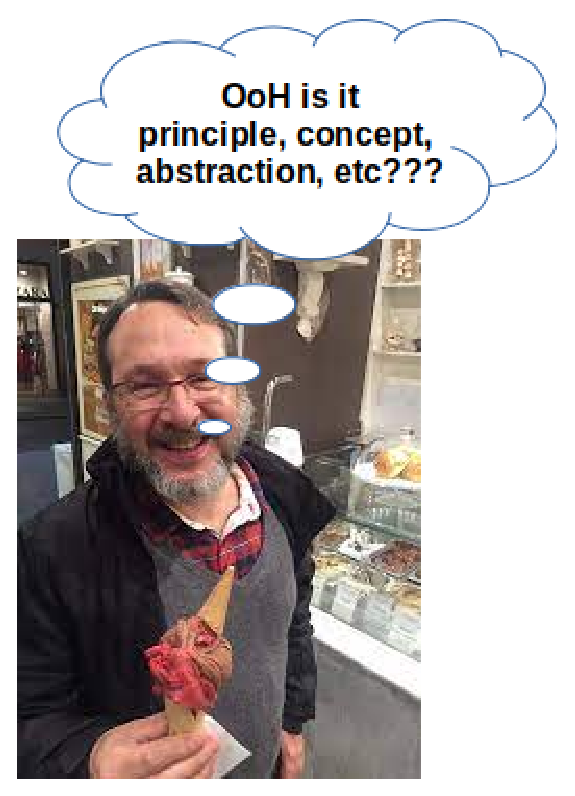
\includegraphics[width=.3\columnwidth]{fig/mullerization}
			\end{figure}         
        \end{frame} 
%%%%%%%%%%%%%%%%%%%%%%%%%%%%%%%%%%%%%%%%%%%%%%%%%%%%%%%%%%%%%%%%%%%%%%%%%%%%%%%%%%%
        \begin{frame}
        \frametitle{Muller-ization} 
 		    \begin{figure}
			\centering
	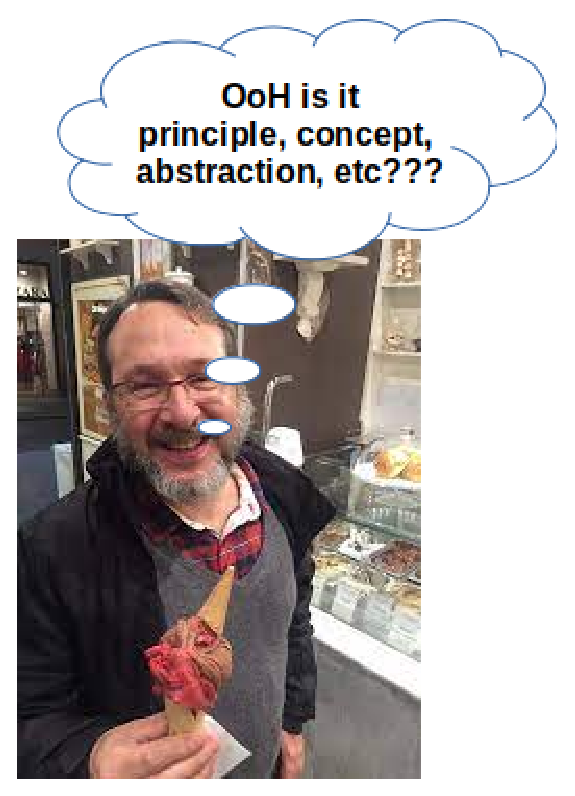
\includegraphics[width=.2\columnwidth]{fig/mullerization}
			\end{figure}         
				\begin{itemize}
					\item \huge OoH is about a new research axis
				\end{itemize}
        \end{frame}               
%%%%%%%%%%%%%%%%%%%%%%%%%%%%%%%%%%%%%%%%%%%%%%%%%%%%%%%%%%%%%%%%%%%%%%%%%%%%%%%%%%%
        \begin{frame}
        \frametitle{OoH in the design space} 
 		    \begin{figure}
			\centering
	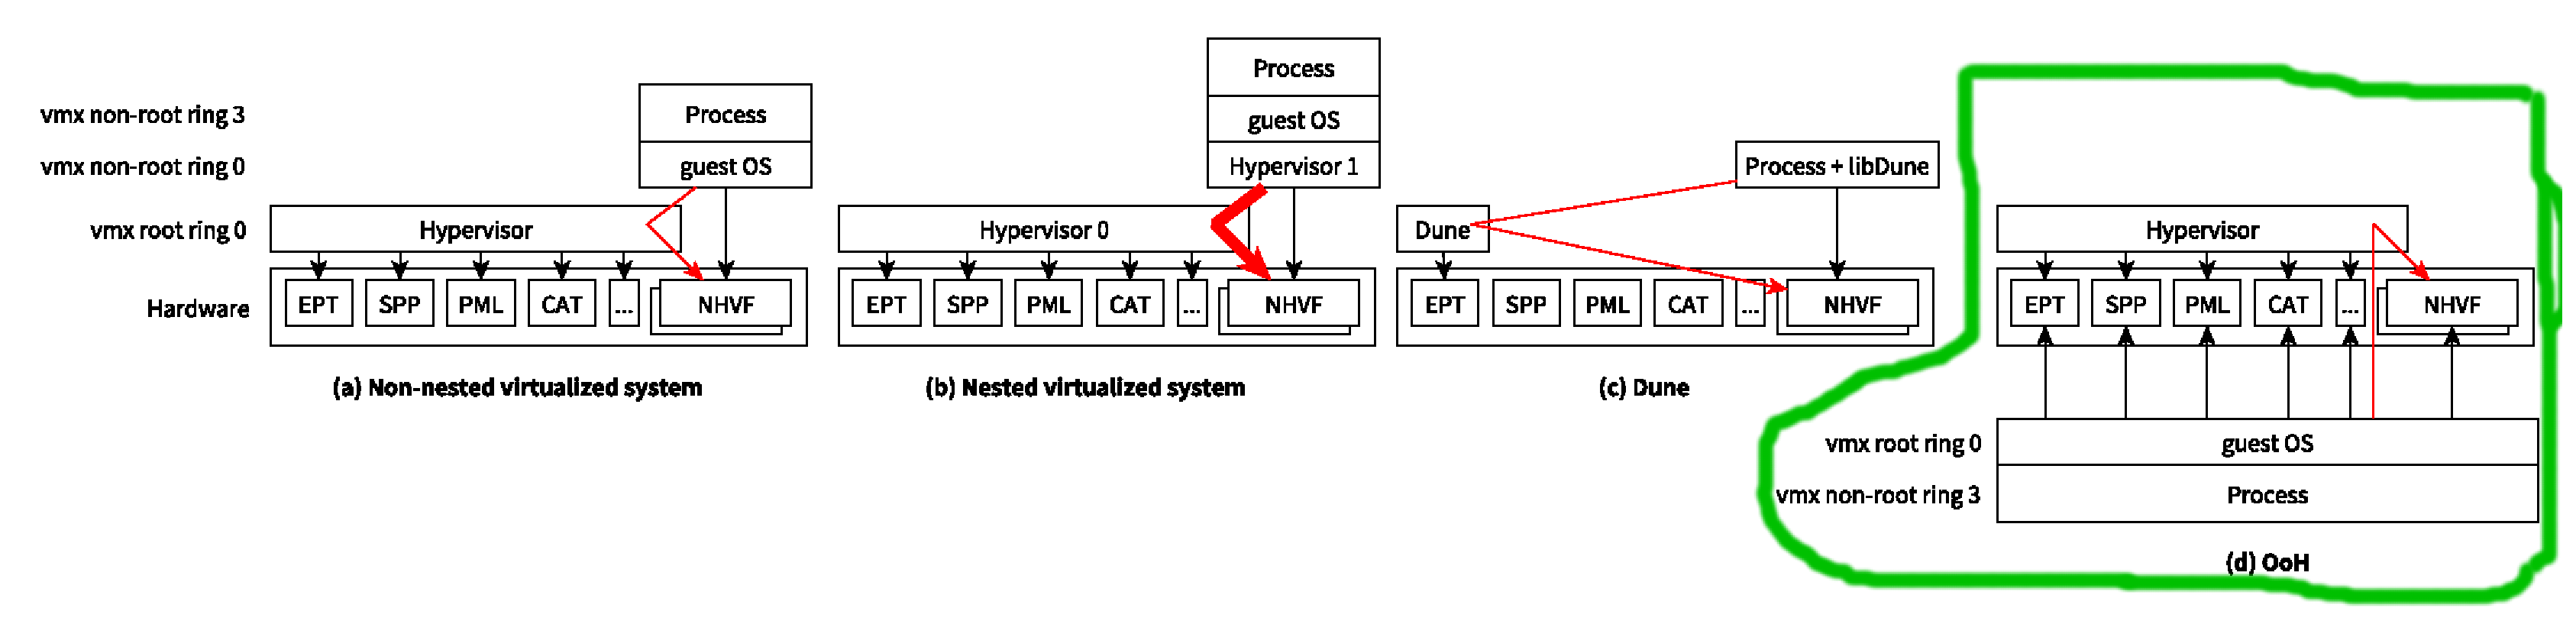
\includegraphics[width=1\columnwidth]{fig/differences}
%	\caption{The position of OoH (d) in the virtualization landscape: (a) non-nested virtualization, (b) nested virtualization (including DVH~\cite{lim.dvh.asplos.2020}) and (c) Dune.
%	Red arrows materialize VM traps.
%	Its width indicates the intensity of VM traps.
%	NHVF stands for Non Hardware Virtualization Feature.}
			\end{figure} 
			\scriptsize NHVF = Non Hardware Virtualization Features (e.g., set CR3 register on x86)\\
			~\\
			\scriptsize Dune is A. Belay et al. OSDI'12			
        \end{frame}        
%%%%%%%%%%%%%%%%%%%%%%%%%%%%%%%%%%%%%%%%%%%%%%%%%%%%%%%%%%%%%%%%%%%%%%%%%%%%%%%%%%%
%        \begin{frame}
%        \frametitle{OoH} 
%			\begin{block}{Examples of hypervisor-oriented hardware virtualization}
%				\begin{itemize}
%					\item Intel Page Modification Logging (PML): allows to track dirty pages for accelerating VM live migration and checkpointing
%					\begin{itemize}
%						\item would allow improving process/container checkpointing, GCs, etc.
%					\end{itemize}
%					\item Intel Sub-Page write Protection (SPP)
%					\begin{itemize}
%						\item would allow reducing memory waste in guard page-based secured heap memory allocators
%					\end{itemize}
%					\item Intel Cache Allocation Technology
%					\begin{itemize}
%						\item would allow isolating processes
%					\end{itemize}
%				\end{itemize}
%			\end{block}			
%        \end{frame}
%%%%%%%%%%%%%%%%%%%%%%%%%%%%%%%%%%%%%%%%%%%%%%%%%%%%%%%%%%%%%%%%%%%%%%%%%%%%%%%%%%%
%        \begin{frame}
%        \frametitle{OoH} 
%			\begin{block}{The main message}
%				\begin{itemize}
%					\item To harware manufacturers
%					\begin{itemize}
%						\item When thinking hypervisor-oriented hardware virtualization features, please think how they can be also used by processes from inside VMs, this may need few efforts
%					\end{itemize}
%				\end{itemize}
%			\end{block}			
%        \end{frame}           
%%%%%%%%%%%%%%%%%%%%%%%%%%%%%%%%%%%%%%%%%%%%%%%%%%%%%%%%%%%%%%%%%%%%%%%%%%%%%%%%%%%
        \begin{frame}
        \frametitle{OoH} 
			\begin{block}{Grants}
				\begin{itemize}
					\item Stella Bitchebe
					\begin{itemize}
						\item NEC Student Research Fellowship 2021
						\item Microsoft Research PhD Fellowship 2021
						\item French ANR Scalevisor
					\end{itemize}
				\end{itemize}
			\end{block}			
        \end{frame}                                                    
%%%%%%%%%%%%%%%%%%%%%%%%%%%%%%%%%%%%%%%%%%%%%%%%%%%%%%%%%%%%%%%%%%%%%%%%%%%%%%%%%%%
        \begin{frame}
        \frametitle{This talk illustrates OoH with 2 features} 
			\begin{block}{OoH for Intel SPP}
				\begin{itemize}
					\item to reduce memory overhead of guard page-based secured heap memory allocators
					\item work in progress
					\item by Yves Kone, Augusta Mukam and Stella Bitchebe
				\end{itemize}
			\end{block}
			\begin{block}{OoH for Intel PML}
				\begin{itemize}
					\item to improve process/container checkpointing, concurrent GCs
					\item work completed!
					\item by Stella Bitchebe
				\end{itemize}
			\end{block}				
        \end{frame}
%%%%%%%%%%%%%%%%%%%%%%%%%%%%%%%%%%%%%%%%%%%%%%%%%%%%%%%%%%%%%%%%%%%%%%%%%%%%%%%%%%%
%        \begin{frame}
%        \frametitle{This talk} 
%			\begin{block}{Intel PML results}
%				\begin{itemize}
%					\item donner les résultats majeurs ici
%				\end{itemize}
%			\end{block}
%			\begin{block}{Intel SPP}
%				\begin{itemize}
%					\item Donner le résultat attendu ici
%				\end{itemize}
%			\end{block}				
%        \end{frame}                                                          
%%%%%%%%%%%%%%%%%%%%%%%%%%%%%%%%%%%%%%%%%%%%%%%%%%%%%%%%%%%%%%%%%%%%%%%%%%%%%%%%%%%         
\section{OoH for Intel SPP}
%%%%%%%%%%%%%%%%%%%%%%%%%%%%%%%%%%%%%%%%%%%%%%%%%%%%%%%%%%%%%%%%%%%%%%%%%%%%%%%%%%%
        \begin{frame}
        \frametitle{Intel SPP} 
			\begin{block}{Overview}
				\begin{itemize}
					\item EPT-based, 4KB page size, organised into 32 sub-pages (128 B each)
				\end{itemize}
			\end{block}
 		    \begin{figure}
			\centering
				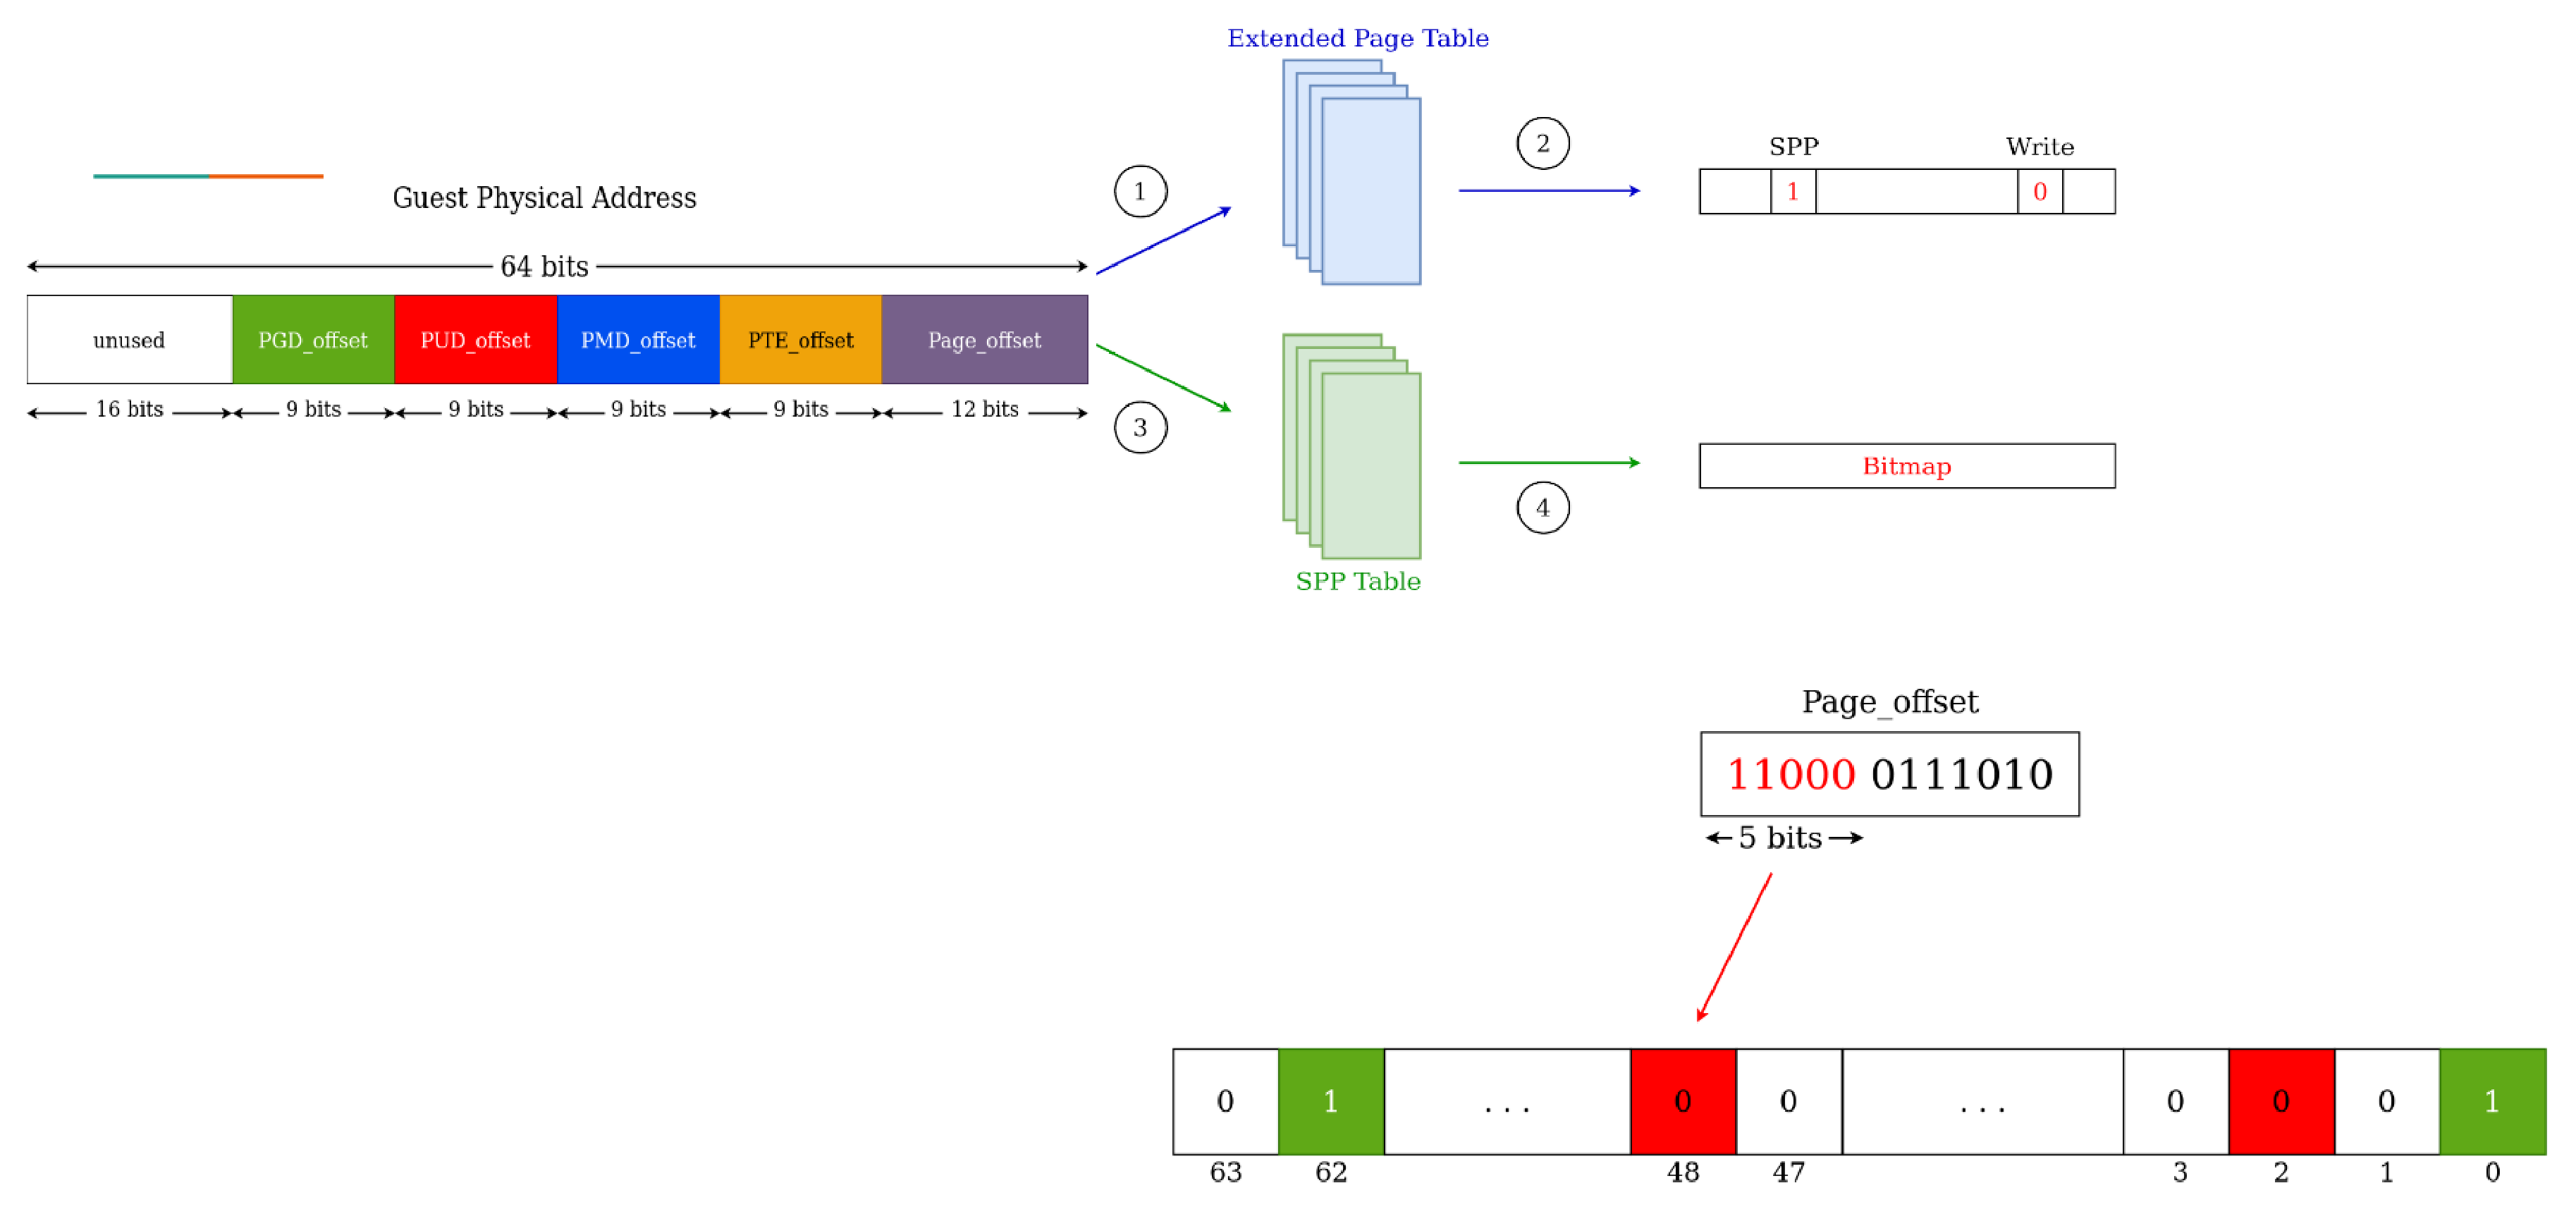
\includegraphics[width=.8\columnwidth]{fig/spp}
%				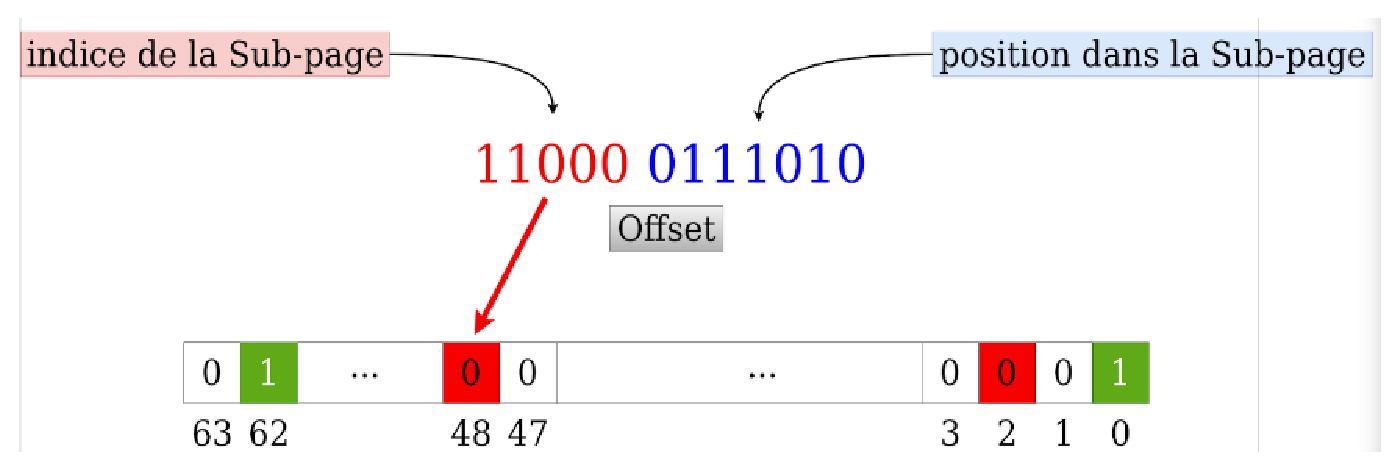
\includegraphics[width=.4\columnwidth]{fig/spp2}				
			\end{figure}			
        \end{frame}
%%%%%%%%%%%%%%%%%%%%%%%%%%%%%%%%%%%%%%%%%%%%%%%%%%%%%%%%%%%%%%%%%%%%%%%%%%%%%%%%%%%
        \begin{frame}
        \frametitle{Buffer overflow vulerability} 
			\begin{block}{Unsafe languages such as C}
 		    \begin{figure}
			\centering
				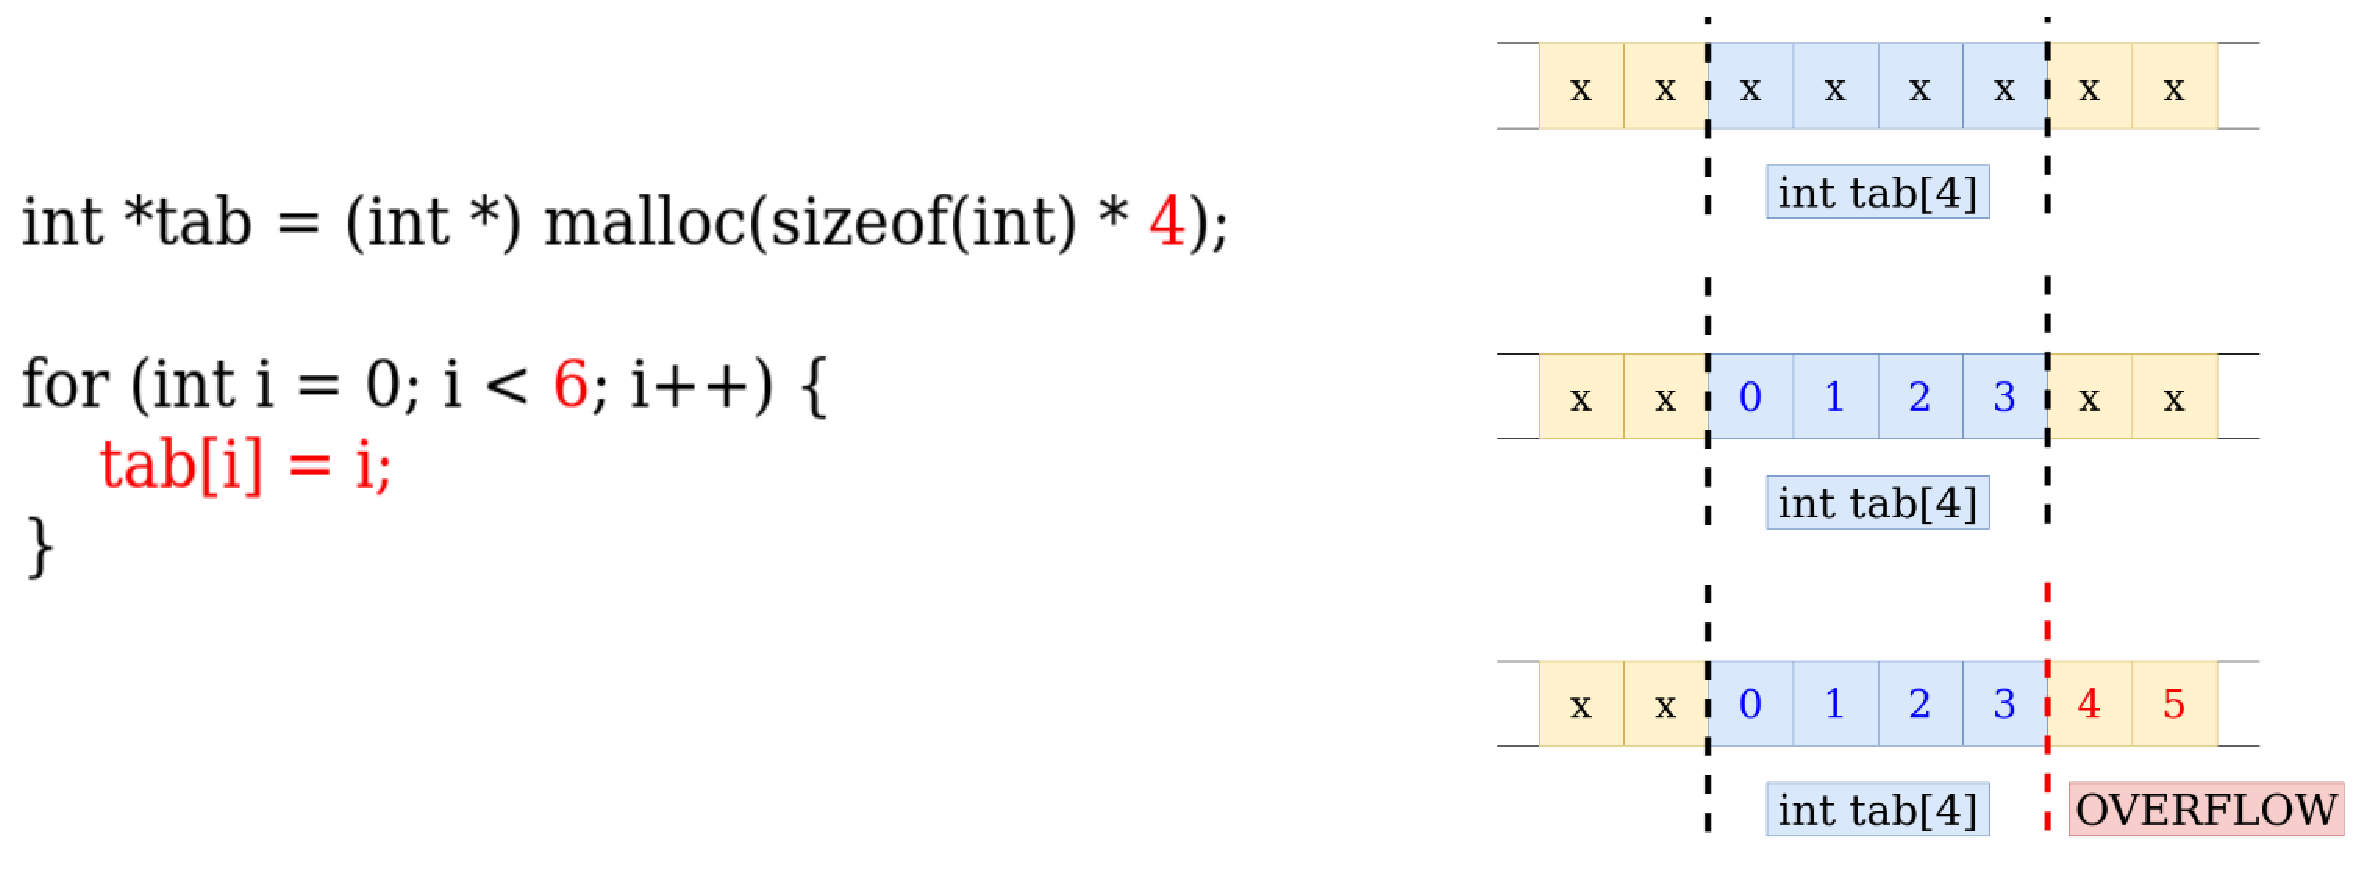
\includegraphics[width=1\columnwidth]{fig/overflow}
			\end{figure}	
			\end{block}		
        \end{frame}      
%%%%%%%%%%%%%%%%%%%%%%%%%%%%%%%%%%%%%%%%%%%%%%%%%%%%%%%%%%%%%%%%%%%%%%%%%%%%%%%%%%%
        \begin{frame}
        \frametitle{Buffer overflow vulerability} 
			\begin{block}{Guard pages}
 		    \begin{figure}
			\centering
				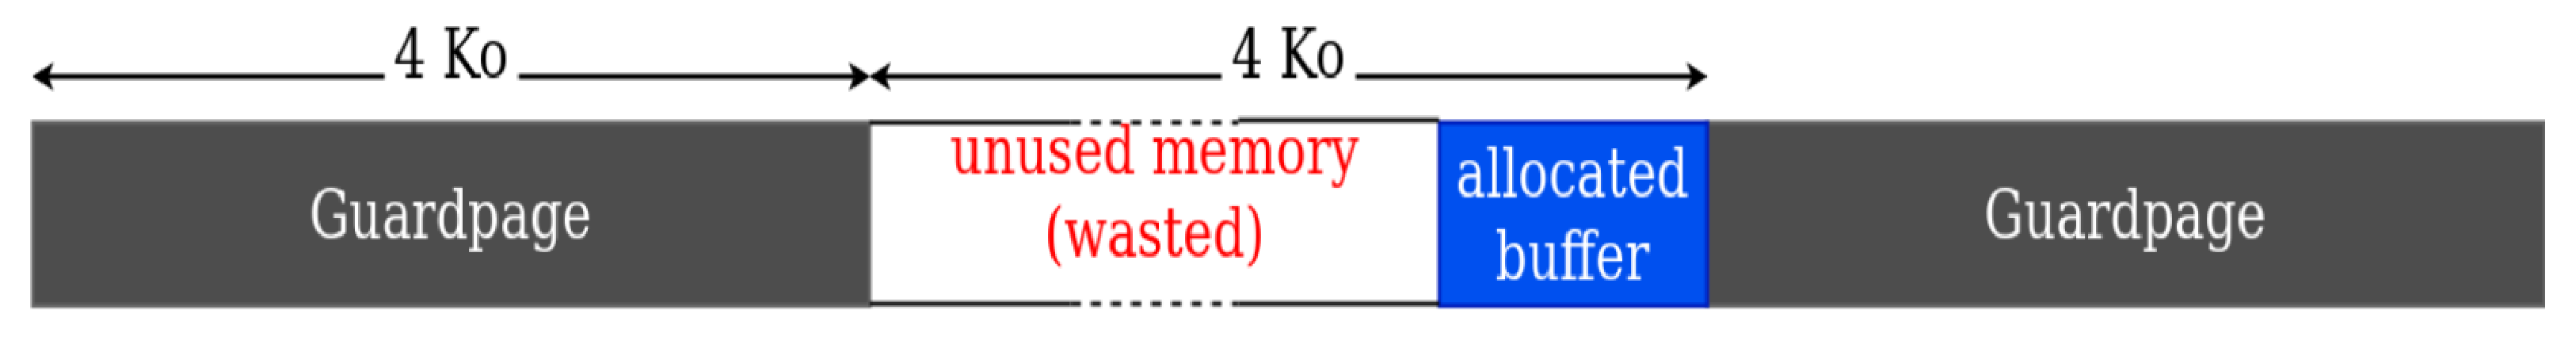
\includegraphics[width=.7\columnwidth]{fig/guard}
			\end{figure}			
				\begin{itemize}
					\item Avantage: sync detection
					\item Limitations: memory waste
				\end{itemize}
			\end{block}		
        \end{frame}           
%%%%%%%%%%%%%%%%%%%%%%%%%%%%%%%%%%%%%%%%%%%%%%%%%%%%%%%%%%%%%%%%%%%%%%%%%%%%%%%%%%%
        \begin{frame}
        \frametitle{Buffer overflow vulerability} 
			\begin{block}{Canari}
 		    \begin{figure}
			\centering
				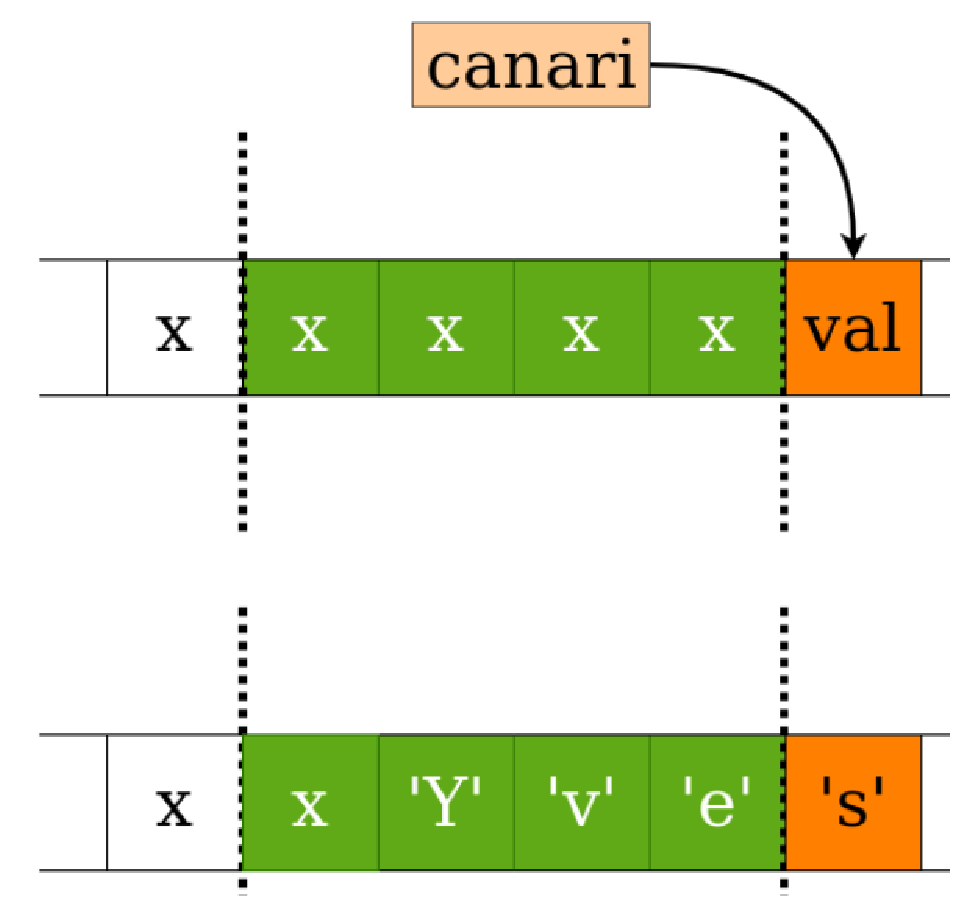
\includegraphics[width=.3\columnwidth]{fig/canari}
			\end{figure}			
				\begin{itemize}
					\item Avantage: low memory waste
					\item Limitations: asyn detection
				\end{itemize}
			\end{block}		
        \end{frame}
%%%%%%%%%%%%%%%%%%%%%%%%%%%%%%%%%%%%%%%%%%%%%%%%%%%%%%%%%%%%%%%%%%%%%%%%%%%%%%%%%%%
        \begin{frame}
        \frametitle{OoH for Intel SPP: Sub guard pages} 
			\begin{block}{overview}
 		    \begin{figure}
			\centering
				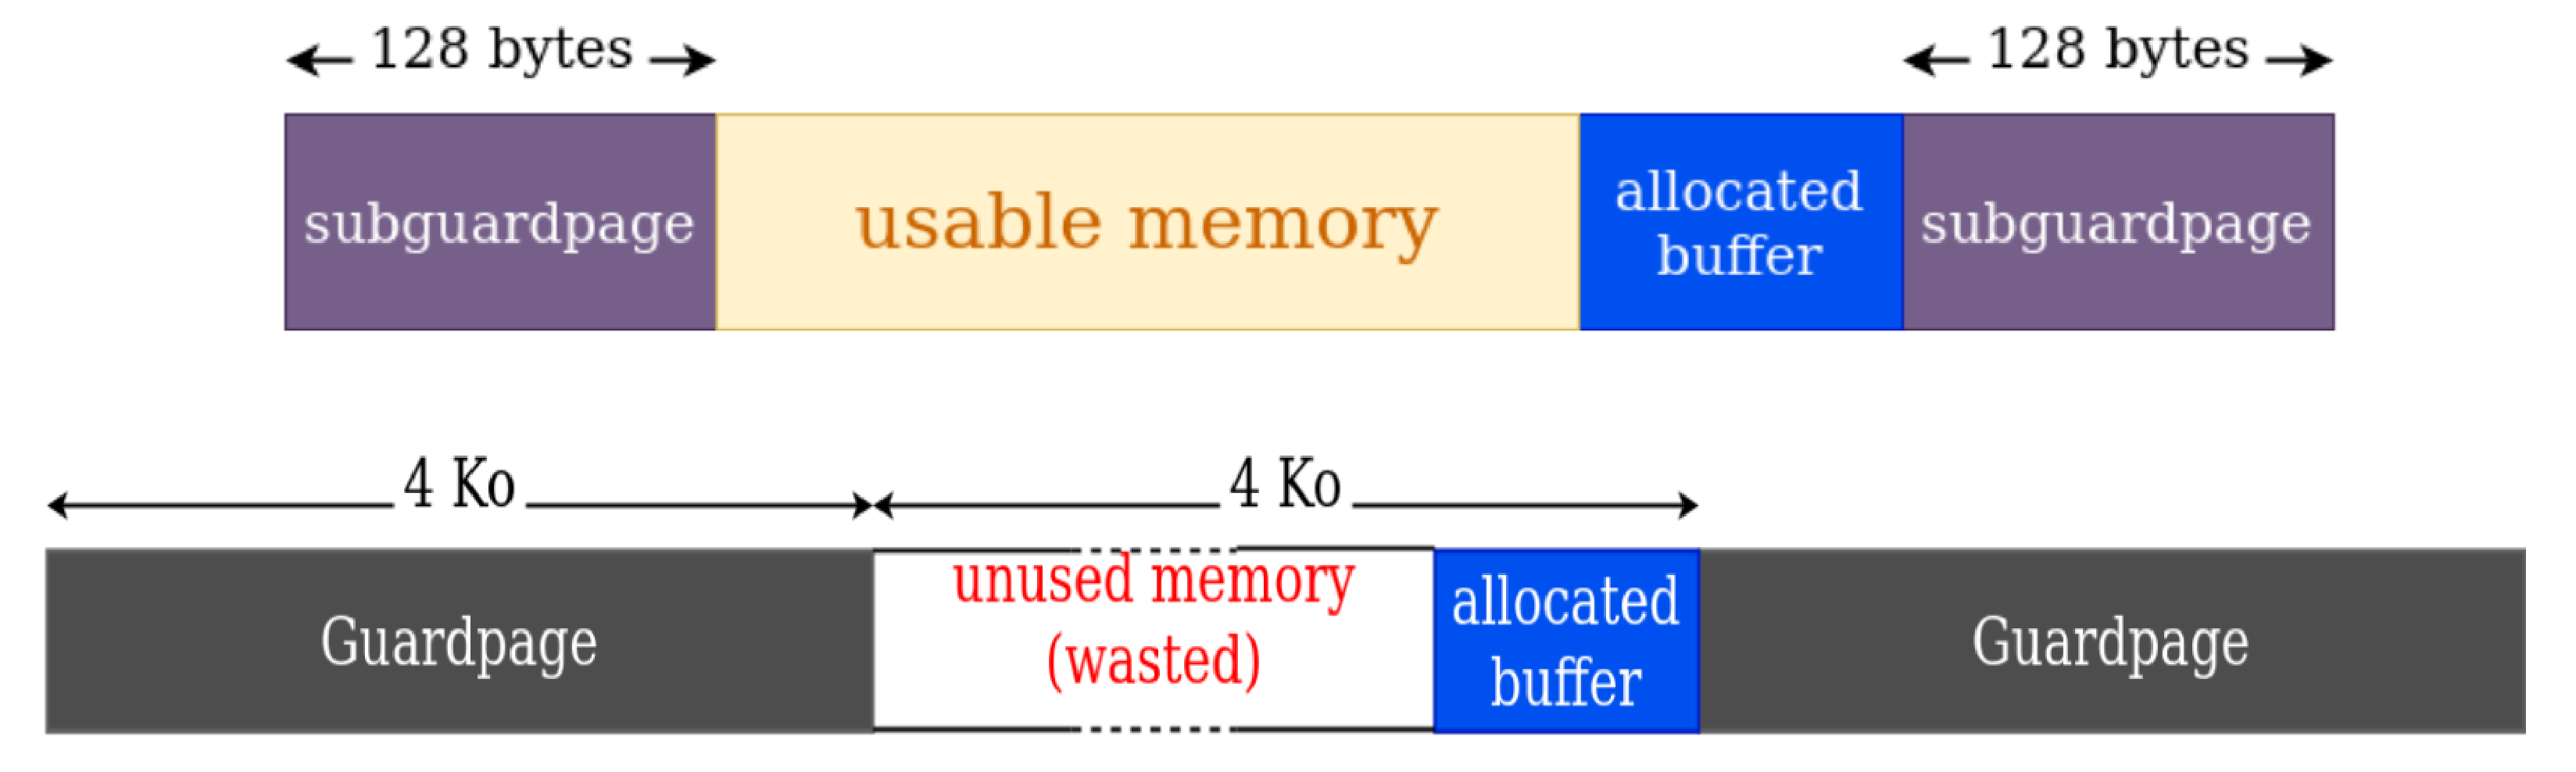
\includegraphics[width=1\columnwidth]{fig/spp-overflow}
			\end{figure}			
				\begin{itemize}
					\item Avantage: sync detection, low memory waste (maximum 128KB instead of 4KB $\rightarrow$ 32$\times$)
				\end{itemize}
			\end{block}		
        \end{frame}   
%%%%%%%%%%%%%%%%%%%%%%%%%%%%%%%%%%%%%%%%%%%%%%%%%%%%%%%%%%%%%%%%%%%%%%%%%%%%%%%%%%%
        \begin{frame}
        \frametitle{OoH for Intel SPP: Sub guard pages}
			\begin{block}{Challenges}			
				\begin{itemize}
					\item SPP is only managed by the hypervisor
					\item A naive solution would lead to several costly hypercalls
				\end{itemize}
			\end{block}	
 		    \begin{figure}
			\centering
				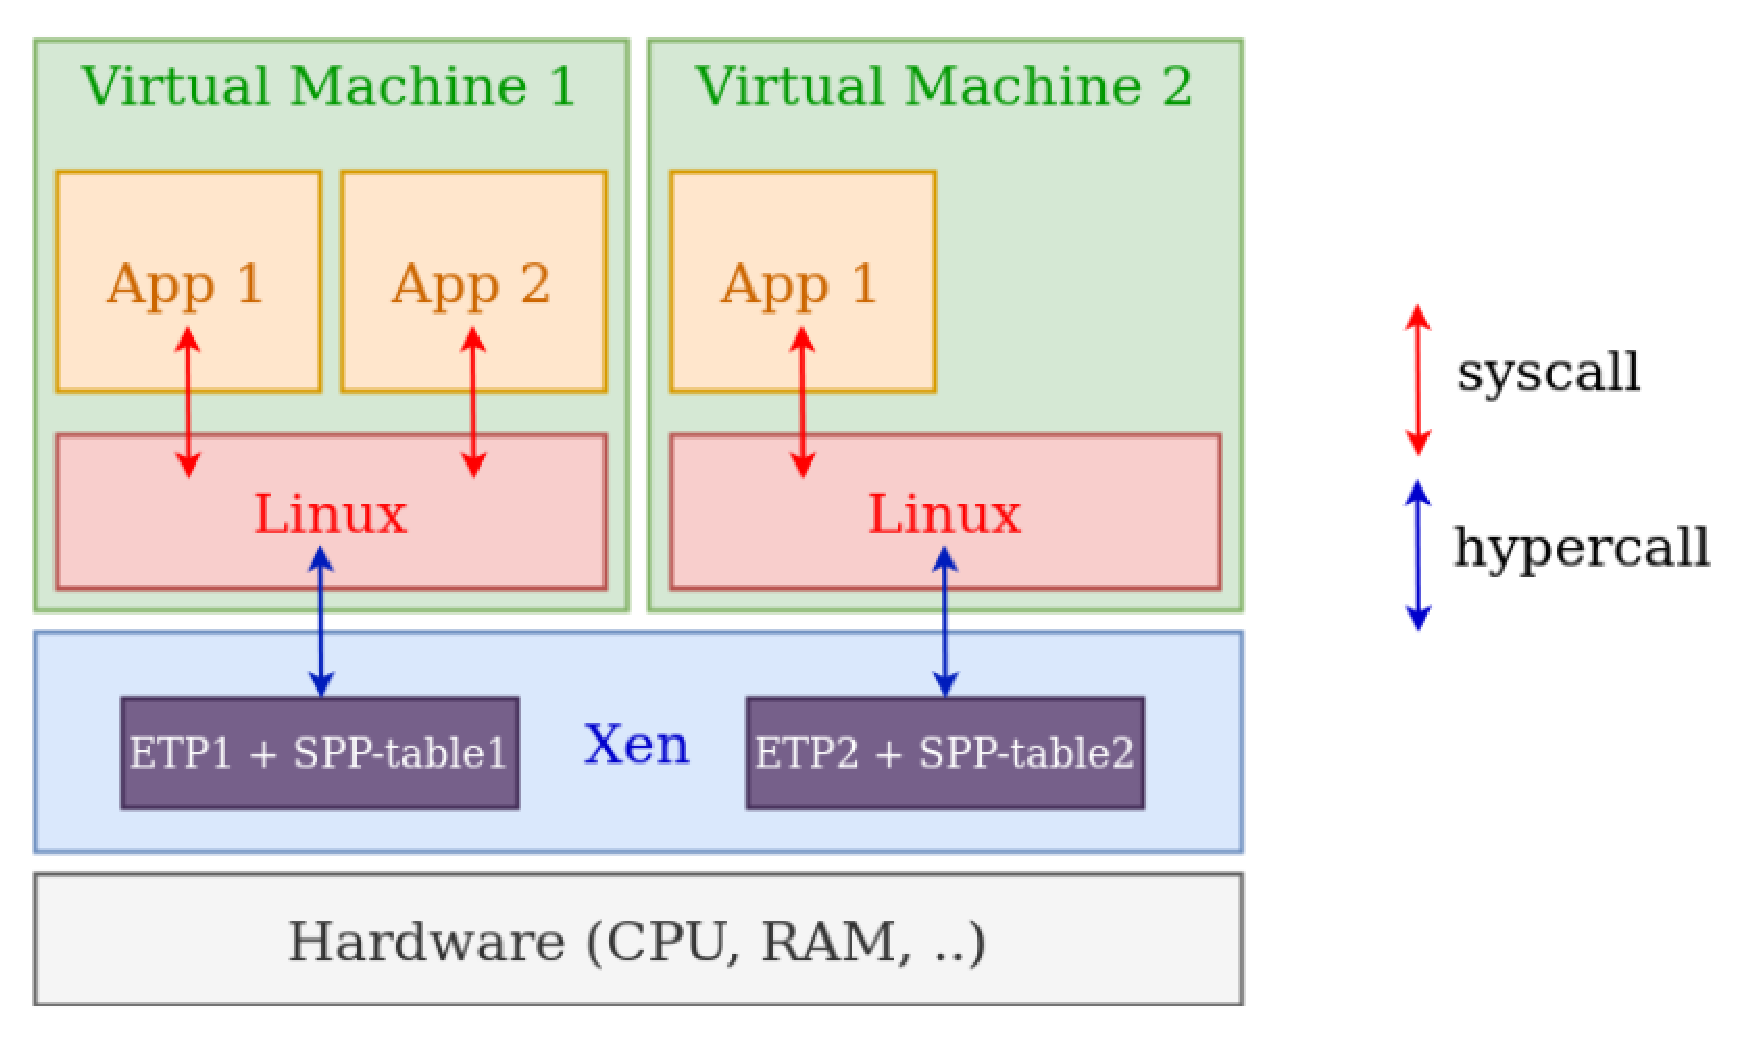
\includegraphics[width=.5\columnwidth]{fig/s0}
			\end{figure}				
        \end{frame}
%%%%%%%%%%%%%%%%%%%%%%%%%%%%%%%%%%%%%%%%%%%%%%%%%%%%%%%%%%%%%%%%%%%%%%%%%%%%%%%%%%%
        \begin{frame}
        \frametitle{OoH for Intel SPP: Sub guard pages} 
			\begin{block}{Approach: Pre-initialized SPP page pool}			
				\begin{itemize}
					\item On demand allocation of pre-initialized SPP pages
					\begin{itemize}
						\item with different write protected sub-page frequencies
					\end{itemize}
				\end{itemize}
			\end{block}	
 		    \begin{figure}
			\centering
				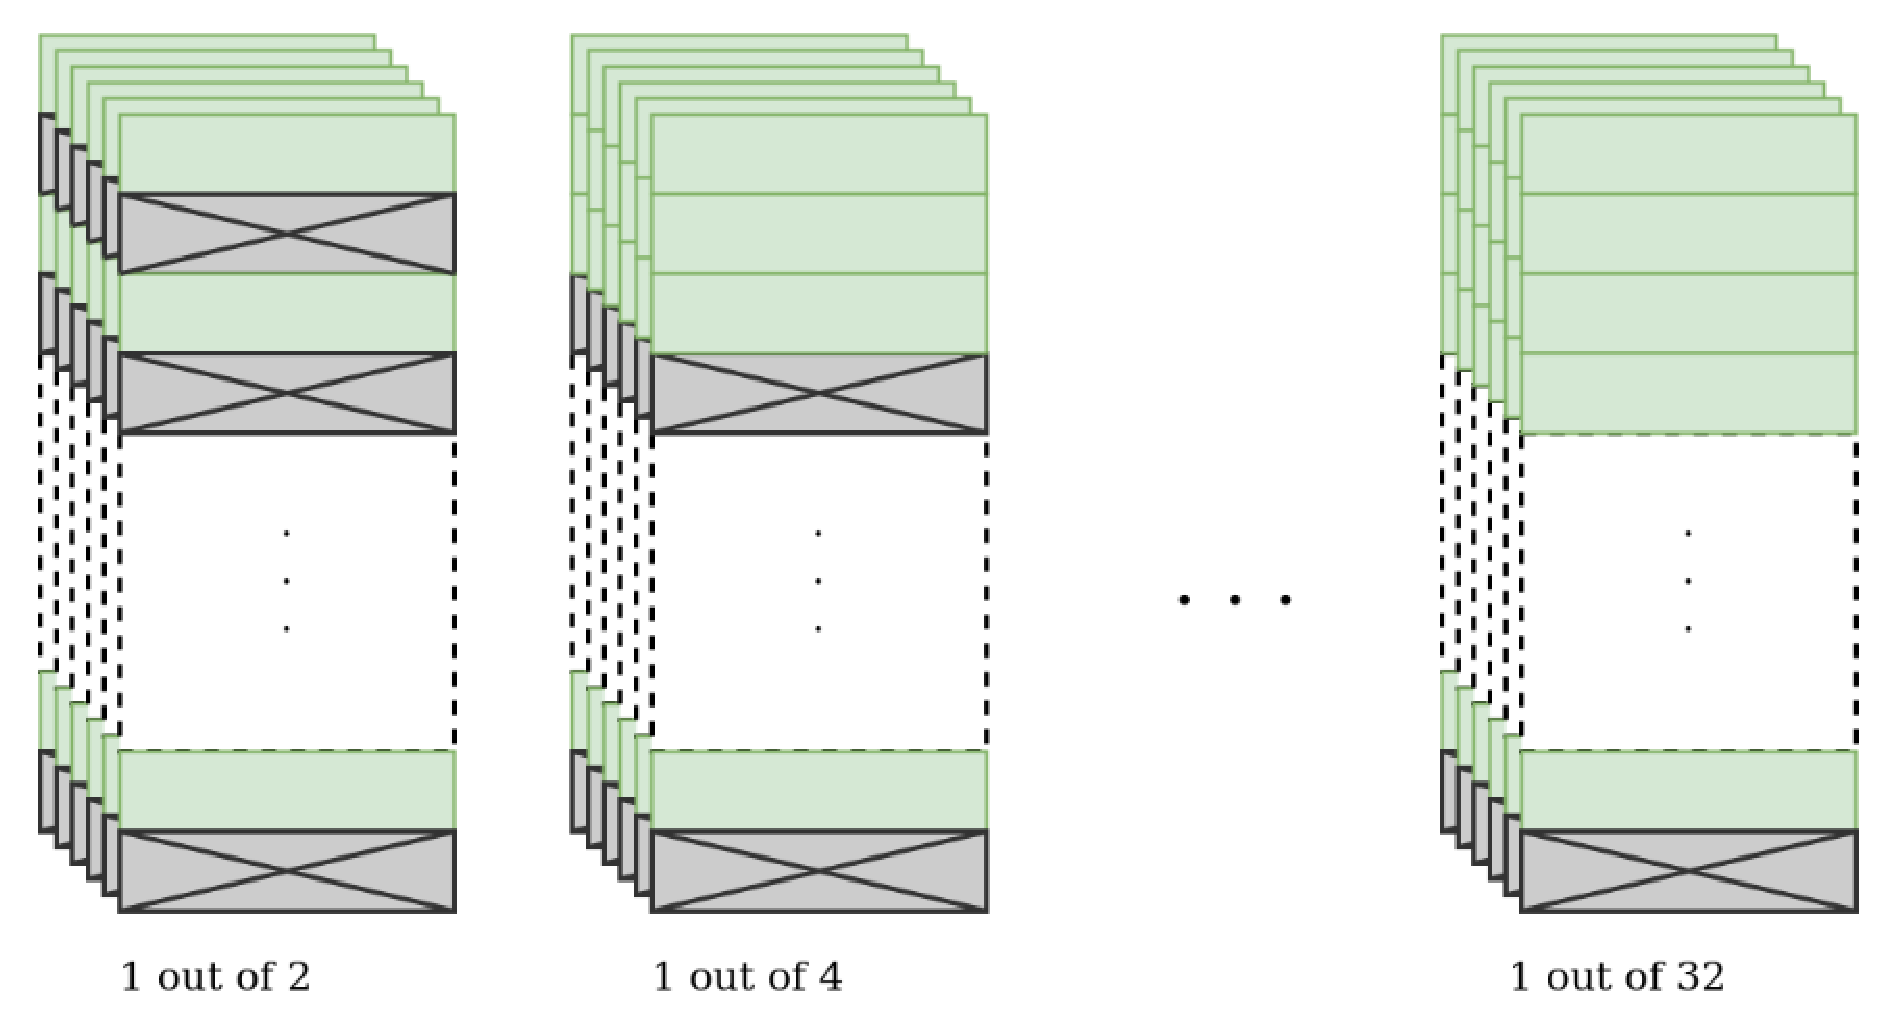
\includegraphics[width=.6\columnwidth]{fig/pool}
			\end{figure}				
        \end{frame}          
%%%%%%%%%%%%%%%%%%%%%%%%%%%%%%%%%%%%%%%%%%%%%%%%%%%%%%%%%%%%%%%%%%%%%%%%%%%%%%%%%%%
%%%%%%%%%%%%%%%%%%%%%%%%%%%%%%%%%%%%%%%%%%%%%%%%%%%%%%%%%%%%%%%%%%%%%%%%%%%%%%%%%%%\\
%%%%%%%%%%%%%%%%%%%%%%%%%%%%%%%%%%%%%%%%%%%%%%%%%%%%%%%%%%%%%%%%%%%%%%%%%%%%%%%%%%%\\
%%%%%%%%%%%%%%%%%%%%%%%%%%%%%%%%%%%%%%%%%%%%%%%%%%%%%%%%%%%%%%%%%%%%%%%%%%%%%%%%%%%
        \begin{frame}
        \frametitle{OoH for Intel SPP: Sub guard pages} 
			\begin{block}{In the guest kernel}			
				\begin{itemize}
					\item Addition of a new memory allocator: for SPP pages
					\item \texttt{struct page *spp\_get\_page(int freq)}: allocate an SPP pre-initialized page
					\item \texttt{int spp\_put\_page(struct page *page, int freq)}: the inverse
					\item Some VMAs are tagged spp
					\item New \texttt{madvise} flags: MADV\_SPP2,...,MADV\_SPP32
				\end{itemize}
			\end{block}					
        \end{frame} 
%%%%%%%%%%%%%%%%%%%%%%%%%%%%%%%%%%%%%%%%%%%%%%%%%%%%%%%%%%%%%%%%%%%%%%%%%%%%%%%%%%%
        \begin{frame}
        \frametitle{OoH for Intel SPP: Sub guard pages} 
			\begin{block}{In the heap memory alocator (e.g., Slimguard)}			
				\begin{itemize}					
					\item \texttt{mmap} a buffer, which creates a new VMA
					\item \texttt{madvise} the buffer using MADV\_SPP2,..., or MADV\_SPP32
					\item use that buffer to allocate secured malloced buffers 
				\end{itemize}
			\end{block}					
        \end{frame}  
%%%%%%%%%%%%%%%%%%%%%%%%%%%%%%%%%%%%%%%%%%%%%%%%%%%%%%%%%%%%%%%%%%%%%%%%%%%%%%%%%%%
        \begin{frame}
        \frametitle{OoH for Intel SPP: Sub guard pages} 
			\begin{block}{On page fault}			
				\begin{itemize}
					\item Check if the target VMS is tagged SPP
					\item If yes, use the new allocator, else use the default buddy allocator
				\end{itemize}
			\end{block}					
        \end{frame} 
%%%%%%%%%%%%%%%%%%%%%%%%%%%%%%%%%%%%%%%%%%%%%%%%%%%%%%%%%%%%%%%%%%%%%%%%%%%%%%%%%%%
        \begin{frame}
        \frametitle{OoH for Intel SPP: Sub guard pages} 
			\begin{block}{Implementation}			
				\begin{itemize}
					\item Xen hypervisor
					\item Linux guest kernel
					\item Slimguard secured heap memory allocator
				\end{itemize}
			\end{block}					
        \end{frame} 
%%%%%%%%%%%%%%%%%%%%%%%%%%%%%%%%%%%%%%%%%%%%%%%%%%%%%%%%%%%%%%%%%%%%%%%%%%%%%%%%%%%
        \begin{frame}
        \frametitle{OoH for Intel SPP: Sub guard pages} 
			\begin{block}{Evaluations}			
				\begin{itemize}
					\item In progress
					\item We expect
					\begin{itemize}
						\item 32$\times$ memory waste reduction
						\item with no performance overhead
					\end{itemize}
				\end{itemize}
			\end{block}					
        \end{frame}         
%%%%%%%%%%%%%%%%%%%%%%%%%%%%%%%%%%%%%%%%%%%%%%%%%%%%%%%%%%%%%%%%%%%%%%%%%%%%%%%%%%%%
%        \begin{frame}
%        \frametitle{Which buffer to protect} 
%			\begin{block}{Slimguard}			
%				\begin{itemize}
%					\item Random
%					\item 1 buffer per xx
%				\end{itemize}
%			\end{block}					
%        \end{frame}
%%%%%%%%%%%%%%%%%%%%%%%%%%%%%%%%%%%%%%%%%%%%%%%%%%%%%%%%%%%%%%%%%%%%%%%%%%%%%%%%%%%%
%        \begin{frame}
%        \frametitle{Which buffer to protect} 
%			\begin{block}{Another contribution}			
%				\begin{itemize}
%					\item We are investigating a smarter approach
%					\item Study CVE to determine which part of the code is vulnerable
%					\item Organize buffers per sensibility
%					\item close to the protected buffer
%					\item introduction of secure\_malloc() and secure\_free(), dynamically introduced in the code during compilation
%				\end{itemize}
%			\end{block}					
%        \end{frame}
%%%%%%%%%%%%%%%%%%%%%%%%%%%%%%%%%%%%%%%%%%%%%%%%%%%%%%%%%%%%%%%%%%%%%%%%%%%%%%%%%%%%
%        \begin{frame}
%        \frametitle{Which buffer to protect} 
%			\begin{block}{Another contribution}			
%				\begin{itemize}
%					\item Since September: CVE analysis from 2010 to 2021
%					\item hard hard. Not well organized
%					\item we have proposed a systematic methodology, after several months of work
%					\item how to automate CVE analysis?
%				\end{itemize}
%			\end{block}					
%        \end{frame}
%%%%%%%%%%%%%%%%%%%%%%%%%%%%%%%%%%%%%%%%%%%%%%%%%%%%%%%%%%%%%%%%%%%%%%%%%%%%%%%%%%%
%        \begin{frame}
%        \frametitle{Which buffer to protect} 
%			\begin{block}{Analysis algorithm}			
%				\begin{itemize}
%					\item xxx
%				\end{itemize}
%			\end{block}					
%        \end{frame}
%%%%%%%%%%%%%%%%%%%%%%%%%%%%%%%%%%%%%%%%%%%%%%%%%%%%%%%%%%%%%%%%%%%%%%%%%%%%%%%%%%%%
%        \begin{frame}
%        \frametitle{Which buffer to protect} 
%			\begin{block}{Some analysis results}			
%				\begin{itemize}
%					\item xxx
%				\end{itemize}
%			\end{block}					
%        \end{frame}   
%%%%%%%%%%%%%%%%%%%%%%%%%%%%%%%%%%%%%%%%%%%%%%%%%%%%%%%%%%%%%%%%%%%%%%%%%%%%%%%%%%%
        \begin{frame}
        \frametitle{Back to "Some famous cameroonians"} 
 		    \begin{figure}
			\centering
	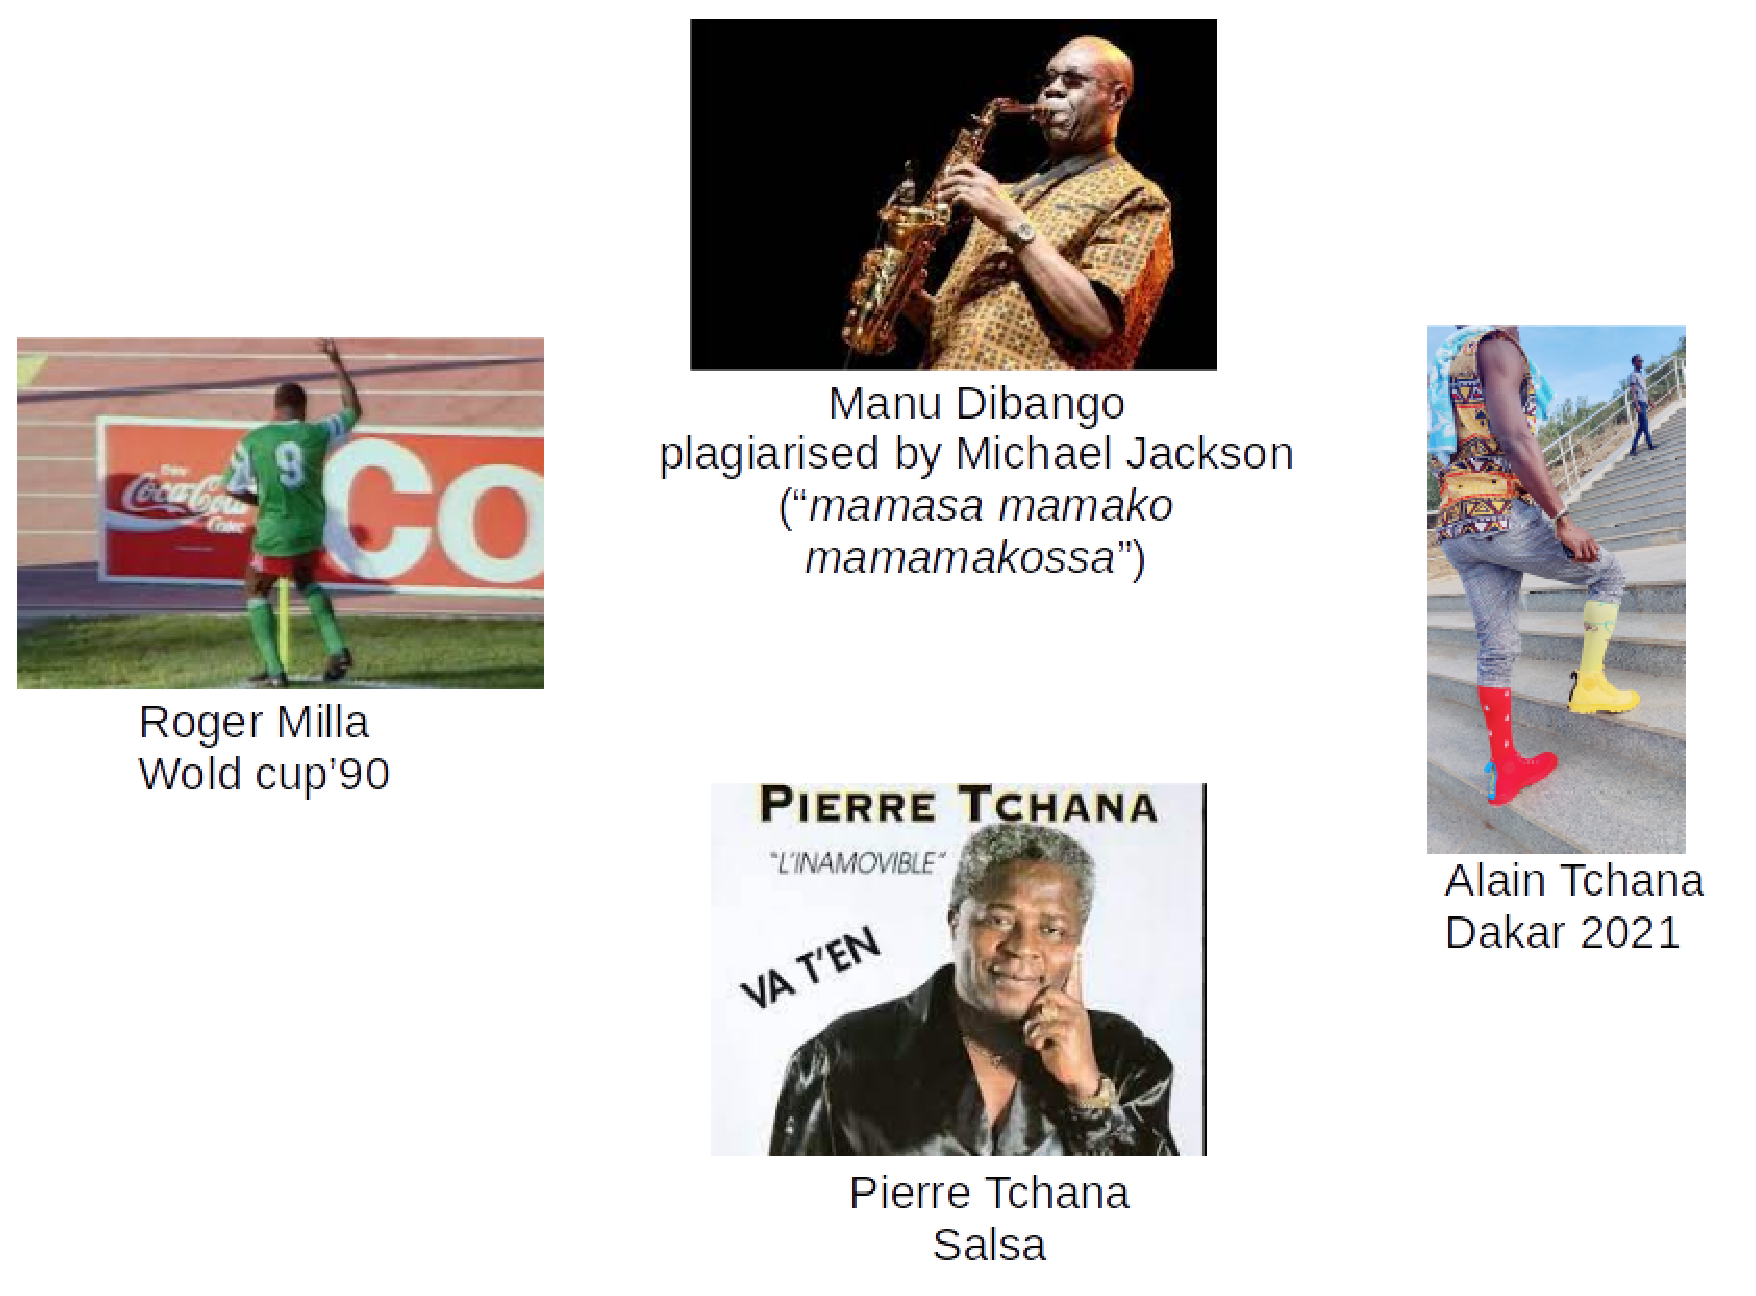
\includegraphics[width=.7\columnwidth]{fig/famous}
			\end{figure}			
        \end{frame}                       
%%%%%%%%%%%%%%%%%%%%%%%%%%%%%%%%%%%%%%%%%%%%%%%%%%%%%%%%%%%%%%%%%%%%%%%%%%%%%%%%%%%         
\section{OoH for Intel PML}
%%%%%%%%%%%%%%%%%%%%%%%%%%%%%%%%%%%%%%%%%%%%%%%%%%%%%%%%%%%%%%%%%%%%%%%%%%%%%%%%%%%
        \begin{frame}
        \frametitle{Intel PML} 
			\begin{block}{Functioning}
 		    \begin{figure}
			\centering
				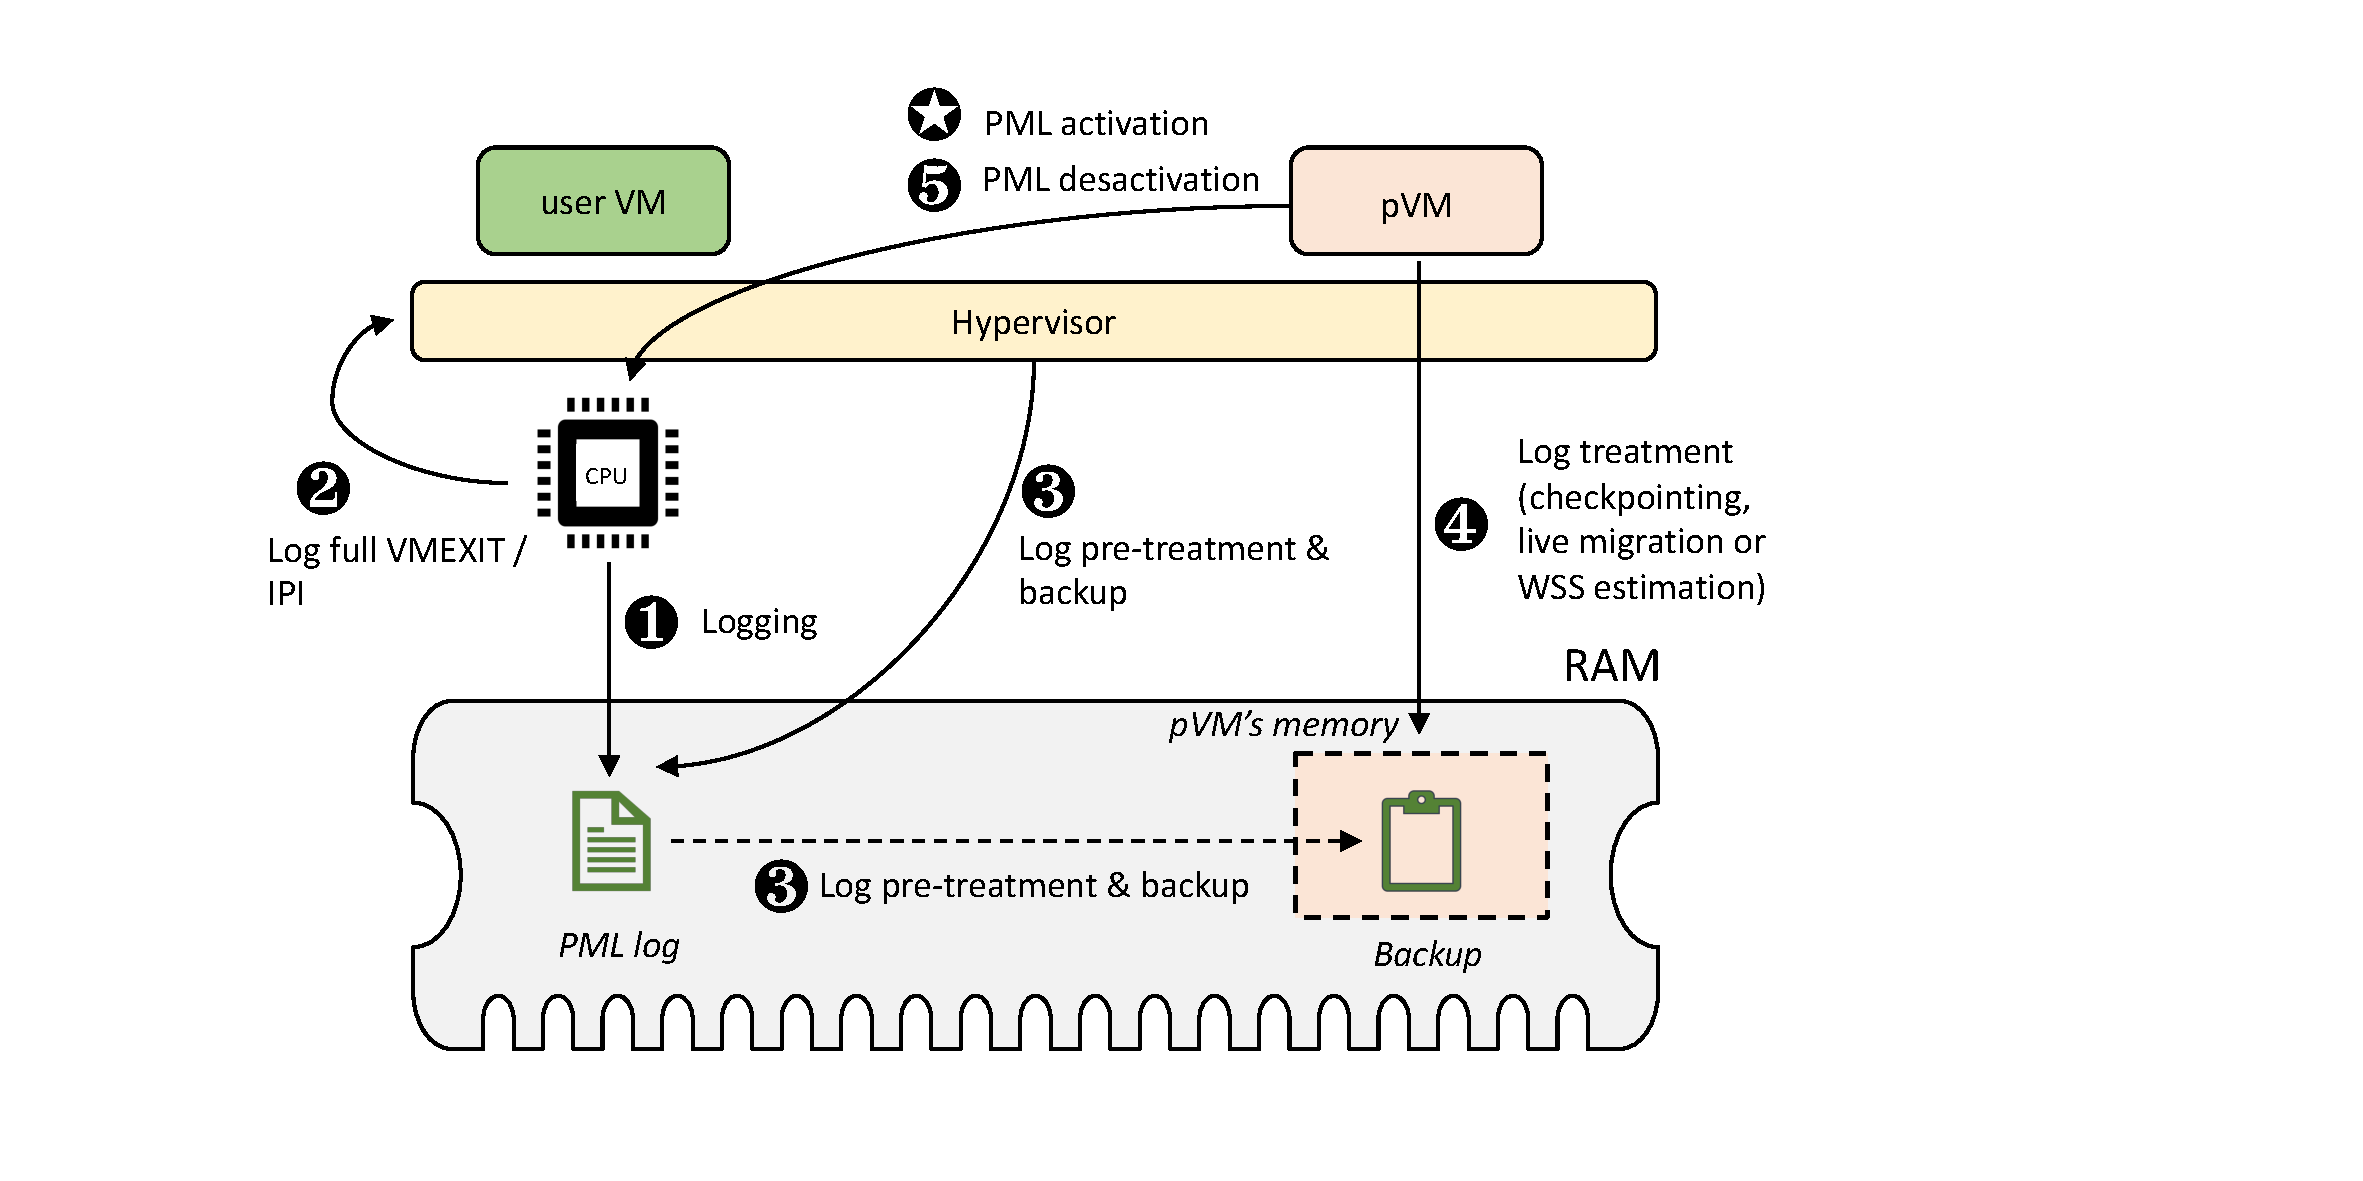
\includegraphics[width=.55\columnwidth]{fig/pmlactualDesign_v2}
			\end{figure}
			\end{block}
			\begin{block}{Intel PML}
				\begin{itemize}
					\item to accelerate CRIU and Boehm GC
				\end{itemize}
			\end{block}				
        \end{frame}
%%%%%%%%%%%%%%%%%%%%%%%%%%%%%%%%%%%%%%%%%%%%%%%%%%%%%%%%%%%%%%%%%%%%%%%%%%%%%%%%%%%
        \begin{frame}
        \frametitle{OoH PML: dirty page tracking in userspace} 
			\begin{block}{Some definitions}
				\begin{itemize}
					\item Tracker: the monitoring thread
					\begin{itemize}
						\item e.g., CRIU, Boehm GC (C and C++ applications)
					\end{itemize}
					\item Tracked: the thread whose memory is monitored
					\begin{itemize}
						\item any application
					\end{itemize}
				\end{itemize}
			\end{block}
			\begin{block}{Current approach}
				\begin{itemize}
					\item page write protection
					\item two main solutions
					\begin{itemize}
						\item bit 55 of /proc/<PID>/pagemap
						\item userfaultfd (ufd)
					\end{itemize}
				\end{itemize}
			\end{block}				
        \end{frame} 
%%%%%%%%%%%%%%%%%%%%%%%%%%%%%%%%%%%%%%%%%%%%%%%%%%%%%%%%%%%%%%%%%%%%%%%%%%%%%%%%%%%
        \begin{frame}
        \frametitle{Dirty page tracking in userspace} 
			\begin{block}{Overall functioning}
				\begin{itemize}
					\item Tracker's activity can be organized in four phases: 
					\begin{itemize}
						\item the initialization of the tracking method,
						\item the monitoring
						\item the collection of dirty page addresses
						\item the exploitation of the latter (e.g., for checkpointing)
					\end{itemize}
				\end{itemize}
			\end{block}
 		    \begin{figure}
			\centering
				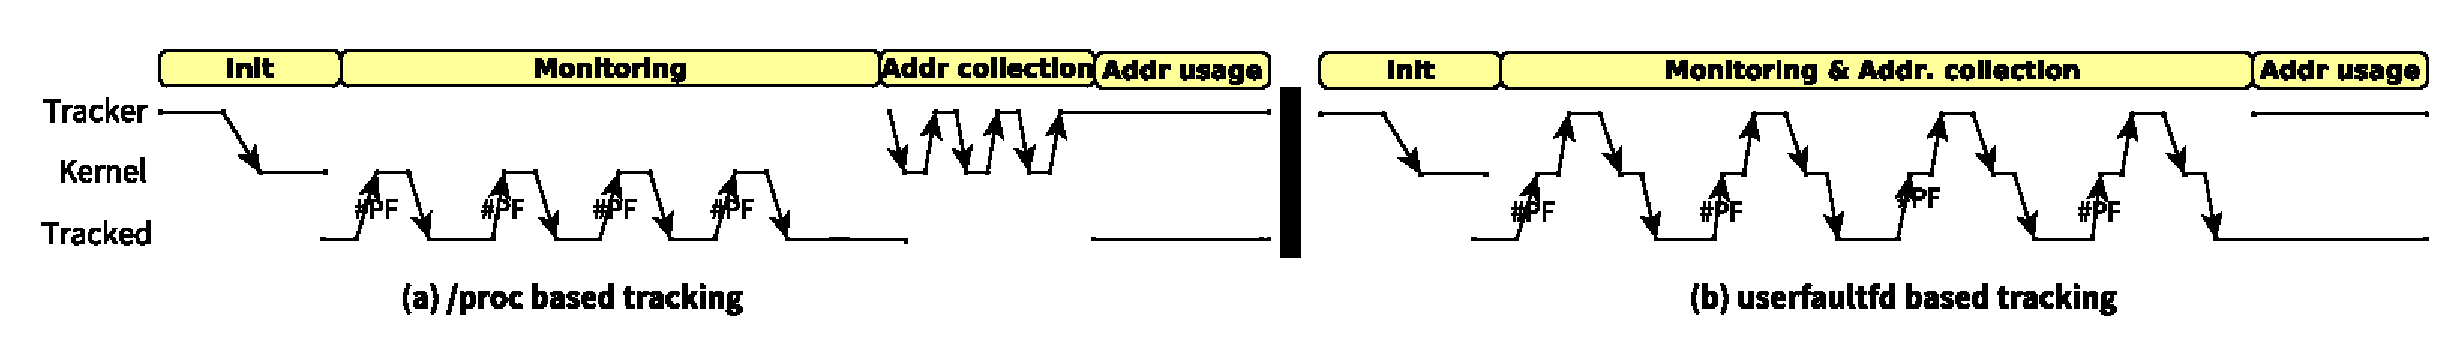
\includegraphics[width=1\columnwidth]{fig/solutions1}
			\end{figure}				
        \end{frame}  
%%%%%%%%%%%%%%%%%%%%%%%%%%%%%%%%%%%%%%%%%%%%%%%%%%%%%%%%%%%%%%%%%%%%%%%%%%%%%%%%%%%
        \begin{frame}
        \frametitle{Dirty page tracking in userspace} 
 		    \begin{figure}
			\centering
				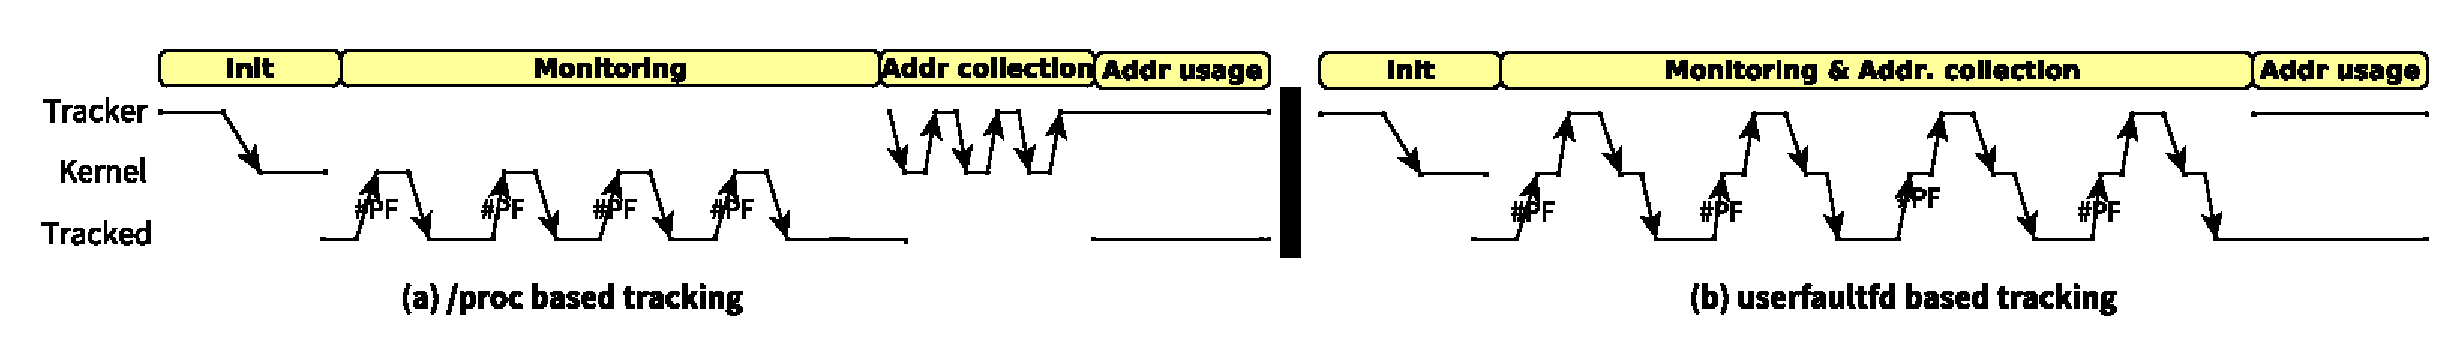
\includegraphics[width=1\columnwidth]{fig/solutions1}
			\end{figure}
~\\			
~\\
 		    \begin{figure}
			\centering
				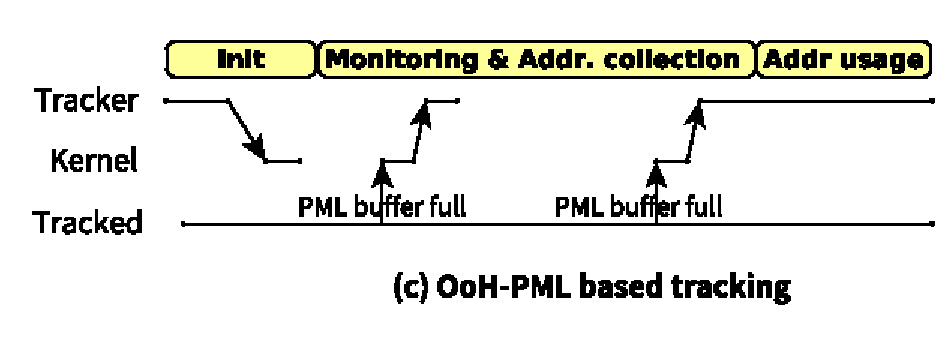
\includegraphics[width=.5\columnwidth]{fig/solutions2}				
			\end{figure}							
        \end{frame}          
%%%%%%%%%%%%%%%%%%%%%%%%%%%%%%%%%%%%%%%%%%%%%%%%%%%%%%%%%%%%%%%%%%%%%%%%%%%%%%%%%%%
        \begin{frame}
        \frametitle{Page write protection} 
			\begin{block}{Limitations}
				\begin{itemize}
					\item ufd 
					\begin{itemize}
						\item we measured an overhead of up to 1,462\% and 1,349\% for 1GB on Tracked and Tracker respectively.% We breakdown the page fault handling time into two components: the time spent inside the kernel (about 33.6ms for 1GB) and the time spent in Tracker (about 3,3383ms for 1GB). The total suspension time of Tracked represents in average about 93\% of its execution time.
						\item due to page fault handling
					\end{itemize}
					\item /proc 
					\begin{itemize}
						\item page table parsing and to flush the TLB (about 2.234ms when the monitored memory is 1GB), soft-dirty bit setting (about 33.5us)
						\item /proc/PID/pagemap parsing in userspace (about 594.187ms for 1GB)						
					\end{itemize}					
				\end{itemize}
			\end{block}				
        \end{frame}                   
%%%%%%%%%%%%%%%%%%%%%%%%%%%%%%%%%%%%%%%%%%%%%%%%%%%%%%%%%%%%%%%%%%%%%%%%%%%%%%%%%%%
%        \begin{frame}
%        \frametitle{Dirty page tracking in userspace: page write protection based approach} 
%%\fcolorbox{white}{white}{
%\begin{table}[h]
%	\scriptsize
%	\centering
%    \resizebox{\columnwidth}{!}
%	{%
%        \begin{tabular}{ |l|r|r|r|r|r|r|r| }
%            \hline
%            On Tracked & 1MB & 10MB & 50MB & 100MB & 250MB & 500MB & 1GB \\ 
%            \hline
%            \texttt{userfaultfd} & 195 & 272 & 583 & 1,050 & 1,266 & 1,462  & 1,463 \\
%            \hline
%            \texttt{/proc} & 104 & 55 & 114 & 208 & 302 & 307 & 335\\
%            \hline
%        \end{tabular}
%    }
%    \par\smallskip
%    \resizebox{\columnwidth}{!}
%	{%
%        \begin{tabular}{ |l|r|r|r|r|r|r|r| }
%            \toprule
%            \hline
%            On Tracker & 1MB & 10MB & 50MB & 100MB & 250MB & 500MB & 1GB \\ 
%            \hline
%            \texttt{userfaultfd} & 93 & 169 & 477 & 940 & 1,269 & 1,153 & 1,349 \\
%            \hline
%            \texttt{/proc} & 47 & 43 & 58 & 148 & 151 & 143 & 147 \\
%            \hline
%        \end{tabular}
%    }
%	\caption{Overhead (in \%) of \texttt{ufd} and \texttt{/proc}.}
%	\label{tab:basic-clearref-overhead}    
%\end{table}
%%}
%        \end{frame}
%%%%%%%%%%%%%%%%%%%%%%%%%%%%%%%%%%%%%%%%%%%%%%%%%%%%%%%%%%%%%%%%%%%%%%%%%%%%%%%%%%%
        \begin{frame}
                \frametitle{OoH for PML}			
			\begin{block}{Challenges}
				\begin{itemize}
					\item ($C_1$) PML can only be managed by the hypervisor
					\item ($C_2$) PML now works at coarse-grained, that is it concerns the entire VM.
					\item ($C_3$) PML only logs GPA.
				\end{itemize}
			\end{block} 
        \end{frame}         
%%%%%%%%%%%%%%%%%%%%%%%%%%%%%%%%%%%%%%%%%%%%%%%%%%%%%%%%%%%%%%%%%%%%%%%%%%%%%%%%%%%
        \begin{frame}
                \frametitle{OoH for PML}			
			\begin{block}{Two solutions}
				\begin{itemize}
					\item Extended PML (EPML): small hardware changes
					\item Shadow PML (SPML): no hardware modification					
					\begin{itemize}
						\item its huge overhead justifies EPML
					\end{itemize}
				\end{itemize}
			\end{block} 
        \end{frame}  
%%%%%%%%%%%%%%%%%%%%%%%%%%%%%%%%%%%%%%%%%%%%%%%%%%%%%%%%%%%%%%%%%%%%%%%%%%%%%%%%%%%
        \begin{frame}
                \frametitle{OoH for PML}	
 		    \begin{figure}
			\centering
\fcolorbox{white}{black}{	                					
				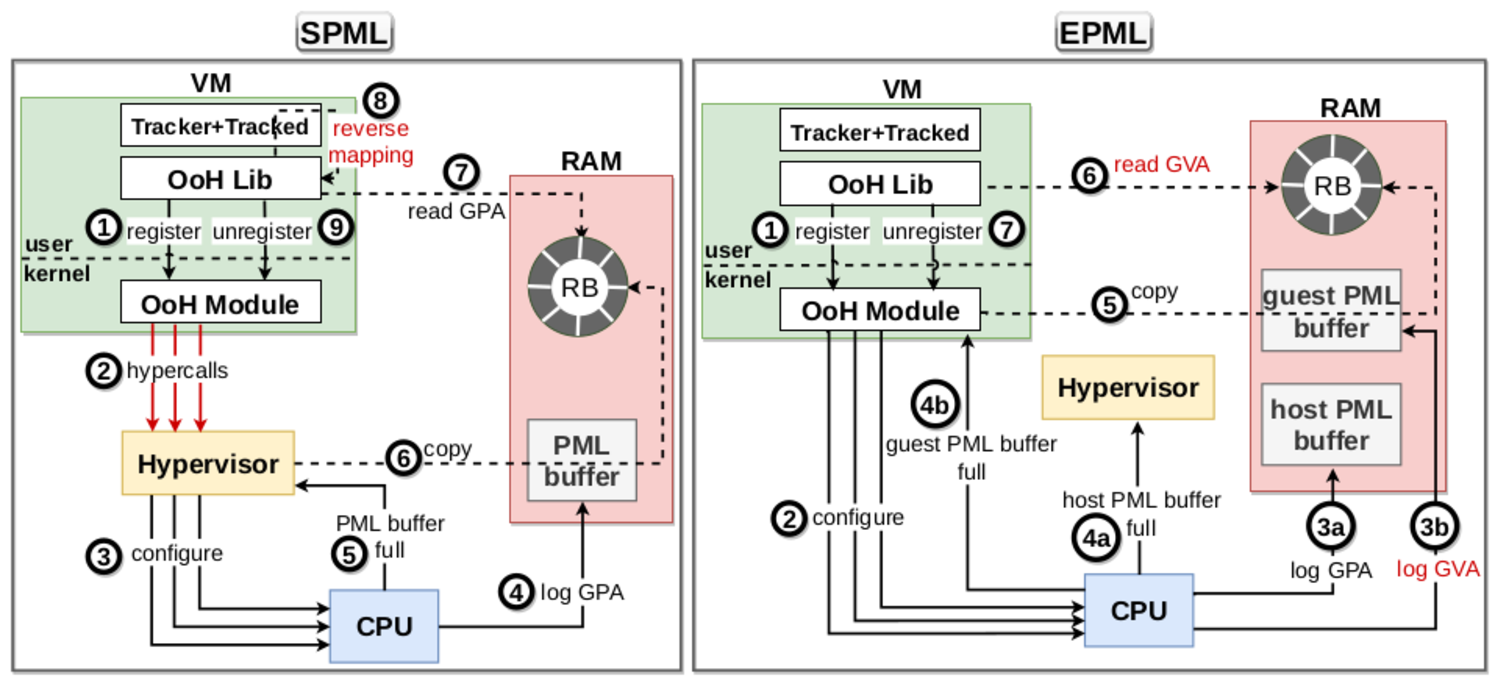
\includegraphics[width=.9\columnwidth]{fig/ooh}
}				
			\end{figure}
        \end{frame}
%%%%%%%%%%%%%%%%%%%%%%%%%%%%%%%%%%%%%%%%%%%%%%%%%%%%%%%%%%%%%%%%%%%%%%%%%%%%%%%%%%%
        \begin{frame}
                \frametitle{OoH for PML}			
			\begin{block}{SPML limitations}
				\begin{itemize}
					\item Costly reverse mapping (takes about $15.739 \: s$ for 1GB working set)
					\item Costly hypercalls ($4.49 \mu s$ to perform an empty hypercall)
				\end{itemize}
			\end{block} 
        \end{frame}
%%%%%%%%%%%%%%%%%%%%%%%%%%%%%%%%%%%%%%%%%%%%%%%%%%%%%%%%%%%%%%%%%%%%%%%%%%%%%%%%%%%
        \begin{frame}
                \frametitle{OoH for PML}			
			\begin{block}{EPML}
				\begin{itemize}
					\item We leverage VMCS shadowing to allow the guest to perform \texttt{vmread} and \texttt{vmwrite} instructions
					\item At load time, OoH Module calls the hypervisor to enable and configure VMCS shadowing
				\end{itemize}
			\end{block} 
        \end{frame} 
%%%%%%%%%%%%%%%%%%%%%%%%%%%%%%%%%%%%%%%%%%%%%%%%%%%%%%%%%%%%%%%%%%%%%%%%%%%%%%%%%%%
        \begin{frame}
                \frametitle{OoH for PML}			
			\begin{block}{Hardware changes}
				\begin{itemize}
					\item We introduce in VMCS's VM-Execution Control area a new field (called \texttt{Guest PML Address})
					\item We extend the page walk to make the processor log GVA to the guest-level PML buffer and the GPA to the hypervisor-level PML buffer.
					\item We modify the hardware so that when the guest-level PML buffer is full, the processor raises a virtual self-IPI (Inter-Processor Interrupt)
				\end{itemize}
			\end{block} 
        \end{frame}     
%%%%%%%%%%%%%%%%%%%%%%%%%%%%%%%%%%%%%%%%%%%%%%%%%%%%%%%%%%%%%%%%%%%%%%%%%%%%%%%%%%%
        \begin{frame}
                \frametitle{OoH for Intel PML}			
			\begin{block}{Implementation}
				\begin{itemize}
					\item We implemented EPML's hardware changes in BOCHS				
					\item We used Xen as the hypervisor and Linux as the guest OS
					\item We integrated OoH Lib with CRIU and Boehm GC
				\end{itemize}
			\end{block} 
        \end{frame}
%%%%%%%%%%%%%%%%%%%%%%%%%%%%%%%%%%%%%%%%%%%%%%%%%%%%%%%%%%%%%%%%%%%%%%%%%%%%%%%%%%%
        \begin{frame}
                \frametitle{OoH for Intel PML}			
			\begin{block}{Evaluations}
				\begin{enumerate}
					\item What is the potential overhead or improvement of SPML and EPML compared to e\texttt{/proc} and \texttt{ufd}?
					\item What is the scalability of SPML and EPML?
				\end{enumerate}
			\end{block} 
        \end{frame}
%%%%%%%%%%%%%%%%%%%%%%%%%%%%%%%%%%%%%%%%%%%%%%%%%%%%%%%%%%%%%%%%%%%%%%%%%%%%%%%%%%%
        \begin{frame}
                \frametitle{OoH for Intel PML}			
			\begin{block}{Methodology}
				\begin{itemize}
					\item We used DELL Intel Core i7-8565U (which provides PML) for experiments				
					\item Micro-benchmarks: Array parsing and GCBench
					\item Macro-benchmarks: tkrzw~\cite{tkrzw} applications (key value store) and Phoenix applications (MapReduce)
					\item We considered three working set sizes (Small, Medium and Large)
				\end{itemize}
			\end{block} 
%\begin{table}%[h]
%	\scriptsize
%	\centering\resizebox{\linewidth}{!}
%	{%
%	\begin{tabular}{ |l|l|c|c|c| }
%		\hline
%		Application & Parameter & Config. small & Config. medium & Config. large \\
%		\toprule\hline
%		GCbench & array size, lived tree depth, stretch tree depth & 500K 16 18 & 650K 18 20 & 750K 20 22 \\
%		\hline
%		histogram & dataset File (GB) & 0.1  & 0.5 & 1.5 \\ 
%		\hline
%		kmeans & d(dimension), c(\#clusters), p(\#points), s(size per dimension) & -d 500 -c 500 -p 500 -p 100 & -d 1K -c 1K -p 1K -s 100 & -d 5K -c 5K -p 5K -s 100 \\
%		\hline
%		matrix-multiply & \#rows, \#columns & 500 500 & 1K 1K & 2K 2K \\
%		\hline
%		pca & r(\#rows), c(\#colums), s(max value) & -r 1K -c 1K -s 200 & -r 5K -c 5K -s 200 & -r 10K -c 10K -s 200 \\
%		\hline
%		string-match & dataset File (MB) & 50 & 100 & 200 \\
%		\hline
%		word-count &  dataset File (MB) & 50 & 100 & 200 \\ 
%		\hline
%	\end{tabular}
%	}
%	\caption{The configuration setup for each Phoenix application and GCbench.}
%	\label{tab:phoenix-gcbench-config}   
%\end{table}
%
%\begin{table}%[bp]
%	%\small
%	\centering
%	\resizebox{\linewidth}{!}
%	{%
%		\begin{tabular}{ |l|l|c|c|c| }
%			\hline
%			Application & Parameter & Config. small & Config. medium & Config. large \\
%			\toprule\hline
%			baby & \#threads, \#iterations & --iter 3M --threads 3 & --iter 5M --threads 3 & --iter 10M --threads 3 \\
%			\hline
%			cache & \#threads, \#iterations, \#records & --iter 3M --cap\_rec\_num 3M --threads 5 & --iter 5M --cap\_rec\_num 5M --threads 5 & --iter 10M --cap\_rec\_num 10M --threads 5 \\ 
%			\hline
%			stdhash & \#threads, \#iterations, mode, \#buckets & --iter 3M --buckets 100K --record\_comp zlib --threads 2 & --iter 5M --buckets 100K --record\_comp zlib --threads 2 & --iter 10M --buckets 100K --record\_comp zlib --threads 2 \\
%			\hline
%			stdtree & \#threads, \#iterations & --iter 3M --threads 2 & --iter 5M --threads 2 & --iter 10M --threads 2 \\
%			\hline
%			tiny & \#threads, \#iterations, \#buckets & --iter 5M --buckets 30M --threads 3 & --iter 5M --buckets 30M --threads 5 & --iter 5M --buckets 30M --threads 7 \\
%			\hline
%		\end{tabular}
%	}
%	\caption{The configuration setup for each tkrzw in-memory engine.}
%	\label{tab:tkrzw-config}   
%\end{table}			
        \end{frame}  
%%%%%%%%%%%%%%%%%%%%%%%%%%%%%%%%%%%%%%%%%%%%%%%%%%%%%%%%%%%%%%%%%%%%%%%%%%%%%%%%%%%
        \begin{frame}
                \frametitle{OoH for Intel PML}			
			\begin{block}{Evaluations}
				\begin{itemize}
					\item How to accurately evaluate EPML?
					\item Approach
					\begin{itemize}
						\item build a formula
						\item show the accuracy of that formula on other techniques, which are measurable
						\item by construction, the formula is accurate for EPML
					\end{itemize}
				\end{itemize}
			\end{block} 
        \end{frame} 
%%%%%%%%%%%%%%%%%%%%%%%%%%%%%%%%%%%%%%%%%%%%%%%%%%%%%%%%%%%%%%%%%%%%%%%%%%%%%%%%%%%
        \begin{frame}
                \frametitle{OoH for Intel PML}			
			\begin{block}{Evaluations}
				\begin{itemize}
					\item The execution time of Tracker when it implements technique $x$
	\begin{equation}
		E(C_{tker}) = E(C_{x}) + E(C_{p}) + I(C_{x},C_{p})
		\label{eq:formula-generic}
	\end{equation}
	where $E(C)$ is the execution time of code $C$ and $I(C_1,C_2)$ is the impact of $C_1$ on $C_2$.
				\end{itemize}
			\end{block} 
        \end{frame}                                                                              
%%%%%%%%%%%%%%%%%%%%%%%%%%%%%%%%%%%%%%%%%%%%%%%%%%%%%%%%%%%%%%%%%%%%%%%%%%%%%%%%%%%  
        \begin{frame}
                \frametitle{Evaluations}
				\begin{block}{Impact on Tracker}
	\begin{equation}\scriptsize
		\begin{split}
			E(C_{/proc}) = & \; E(C_{echo \; 4 \; > \; /proc/PID/clear\_refs}) \\
						& + E(C_{page \; table \; walk \; in \; userspace}) \\
			E(C_{UFD}) = & \; E(C_{ioctl \; write\_protect}) \\
						& + E(C_{ioctl \; register}) \\
						& + E(C_{ioctl \; write\_unprotect}) \\
			E(C_{SPML}) = & \; E(C_{ring \; buffer \; copy}) \\
						& + E(C_{reverse \; mapping}) \\
						& + E(C_{enable/disable \; PML}) \\
			E(C_{EPML}) = & \; E(C_{ring \; buffer \; copy}) \\
						& + E(C_{enable/disable \; PML})
		\end{split}
		\label{eq:formula-detailed}
	\end{equation}								
			\end{block}
        \end{frame}
%%%%%%%%%%%%%%%%%%%%%%%%%%%%%%%%%%%%%%%%%%%%%%%%%%%%%%%%%%%%%%%%%%%%%%%%%%%%%%%%%%%
        \begin{frame}
                \frametitle{OoH for Intel PML}			
			\begin{block}{Evaluations}
				\begin{itemize}
					\item The execution time of Tracked when it is monitored by a tracker using the technique $x$:
	\begin{equation}
		\small
		\label{eq:formula-tracked}
		E(C_{tked\_tker}) = E(C_{tked}) + E(C_{tker}) + I(C_{x},C_{tked})
	\end{equation}
	where $I(C_{x},C_{tked})$ consists of page faults, vmexits, etc..
	Thus, the overhead of $x$ on Tracked is $E(C_{tker}) + I(C_{x},C_{tked})$. 
				\end{itemize}
			\end{block} 
        \end{frame}        
%%%%%%%%%%%%%%%%%%%%%%%%%%%%%%%%%%%%%%%%%%%%%%%%%%%%%%%%%%%%%%%%%%%%%%%%%%%%%%%%%%%
        \begin{frame}
                \frametitle{Evaluations}
				\begin{block}{Impact on Tracked}
	\begin{equation}\scriptsize
		\begin{split}
			I(C_{/proc},C_{tked}) = & \; E(C_{PFH \; in \; kernelspace})\\
									& + E(C_{context \; switch})\\
			I(C_{UFD},C_{tked}) = & \; E(C_{PFH \; in \; userspace})\\
								& + E(C_{context \; switch}) \\
			I(C_{SPML},C_{tked}) = & \; E(C_{vmexits}) \\
								& + N \times E(C_{vmread/vmwrite})\\
			I(C_{EPML},C_{tked}) = & \; N \times E(C_{vmread/vmwrite})	
		\end{split}
		\label{eq:formula-impact-detailed}
	\end{equation}		
For $I(C_{EPML},C_{tked})$, we use SPML's N (the number of context switches) as it is the same (validated by running SPML and EPML under BOCHS).
			\end{block}
        \end{frame}   
%%%%%%%%%%%%%%%%%%%%%%%%%%%%%%%%%%%%%%%%%%%%%%%%%%%%%%%%%%%%%%%%%%%%%%%%%%%%%%%%%%%  
        \begin{frame}
                \frametitle{Formula validation}
\begin{table}[h]
	\centering \scriptsize
	\begin{subtable}[b]{.45\textwidth}
		\centering 
		\begin{tabular}{l l}
			\toprule
			\hline
			Metric & Time (ms) \\
			\hline
			\textcolor{americanrose}{\textbf{$E(C_{tker})$}} & \\
			\textcolor{americanrose}{\textbf{measured}} & \multirow{-2}{*}{\textcolor{americanrose}{\textbf{5503.79}}}\\
			\textcolor{airforceblue}{\textbf{$E(C_{tked\_tker})$}} & \\
			\textcolor{airforceblue}{\textbf{measured}} & \multirow{-2}{*}{\textcolor{airforceblue}{\textbf{135255.35}}}\\
			\midrule
			$E(C_{p})$ & 251.35\\
			$E(C_{copy\_rb})$ & 0.49\\
			$E(C_{disable \; pml})$ & 2.06\\
			$E(C_{rev. \; mapping})$ & 5419 \\
			\textcolor{americanrose}{\textbf{$E(C_{tker})$}}  &\\
			\textcolor{americanrose}{\textbf{estimated}} &  \multirow{-2}{*}{\textcolor{americanrose}{\textbf{5672.9}}}\\
			\midrule
			$E(C_{vmexits})$ & 18000\\
			$N$ & 39\\
			$E(C_{vmread,vmwrite})$ & $1.73 \times 10^{-3}$\\
			\textcolor{airforceblue}{\textbf{$E(C_{tked\_tker})$}}  & \\
			\textcolor{airforceblue}{\textbf{estimated}} & \multirow{-2}{*}{\textcolor{airforceblue}{\textbf{136919.85}}}\\
			\bottomrule
		\end{tabular}
		\subcaption{SPML}
		\label{tab:criu-spml-formula}
	\end{subtable}
	\hfill
	\begin{subtable}[b]{.45\textwidth}
		\centering 
		\begin{tabular}{l l}
			\toprule
			\hline
			Metric & Time (ms) \\
			\hline
			\textcolor{americanrose}{\textbf{$E(C_{tker})$}} & \\
			\textcolor{americanrose}{\textbf{measured}} & \multirow{-2}{*}{\textcolor{americanrose}{\textbf{1097.99}}}\\
			\textcolor{airforceblue}{\textbf{$E(C_{tked\_tker})$}} & \\
			\textcolor{airforceblue}{\textbf{measured}} & \multirow{-2}{*}{\textcolor{airforceblue}{\textbf{115283.98}}}\\
			\midrule
			$E(C_{p})$ & 251.35\\
			$E(C_{clear\_refs})$ & 1.409\\
			$E(C_{PT walk})$ & 0.89\\
			\textcolor{americanrose}{\textbf{$E(C_{tker})$}}  & \\
			\textcolor{americanrose}{\textbf{estimated}} & \multirow{-2}{*}{\textcolor{americanrose}{\textbf{1116.09}}}\\
			\midrule
			$E(C_{PFH user})$ & 0.27\\
			\textcolor{airforceblue}{\textbf{$E(C_{tked\_tker})$}}  &\\
			\textcolor{airforceblue}{\textbf{estimated}} &  \multirow{-2}{*}{\textcolor{airforceblue}{\textbf{114418.58}}}\\
			\bottomrule
		\end{tabular}
		\subcaption{\texttt{/proc}}
		\label{tab:criu-proc-formula}
	\end{subtable}
	\vspace{.3cm}
	\caption{An accuracy of 96.34\% and 99\% respectively}
	\vspace{.3cm}
\end{table}
        \end{frame}  
%%%%%%%%%%%%%%%%%%%%%%%%%%%%%%%%%%%%%%%%%%%%%%%%%%%%%%%%%%%%%%%%%%%%%%%%%%%%%%%%%%%
        \begin{frame}
                \frametitle{Evaluations}
				\begin{block}{Formula validation}
					An accuracy of about 96.34\% and 99\% respectively for SPML and /proc formulas
			\end{block}
        \end{frame}                 
%%%%%%%%%%%%%%%%%%%%%%%%%%%%%%%%%%%%%%%%%%%%%%%%%%%%%%%%%%%%%%%%%%%%%%%%%%%%%%%%%%%
        \begin{frame}
                \frametitle{Evaluations}
				\begin{block}{Micro-benchmark results}
				
\begin{figure}[!h]
	\centering 
	\begin{minipage}[t]{.45\columnwidth}
\fcolorbox{white}{white}{	
		\centering 
		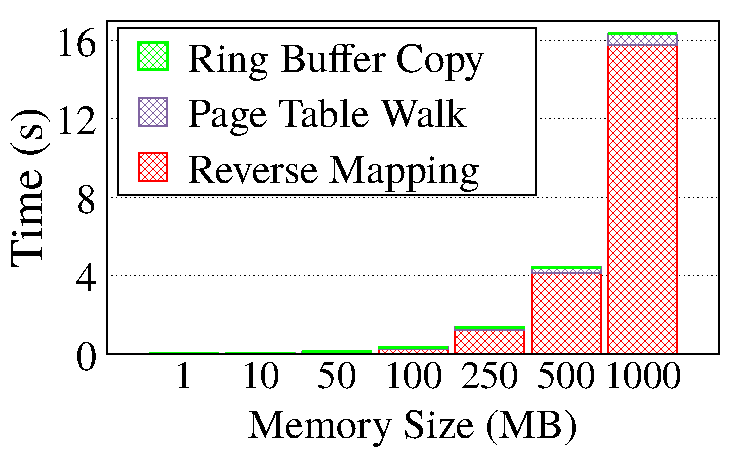
\includegraphics[width=\linewidth]{fig/bottleneck}%
}		
		\captionof{figure}{\small Reverse mapping appears to be the bottleneck of SPML.}
		\label{fig:spml-bottleneck}
	\end{minipage}
	\quad
	\begin{minipage}[t]{.45\columnwidth}
		\centering 
\fcolorbox{white}{white}{		
		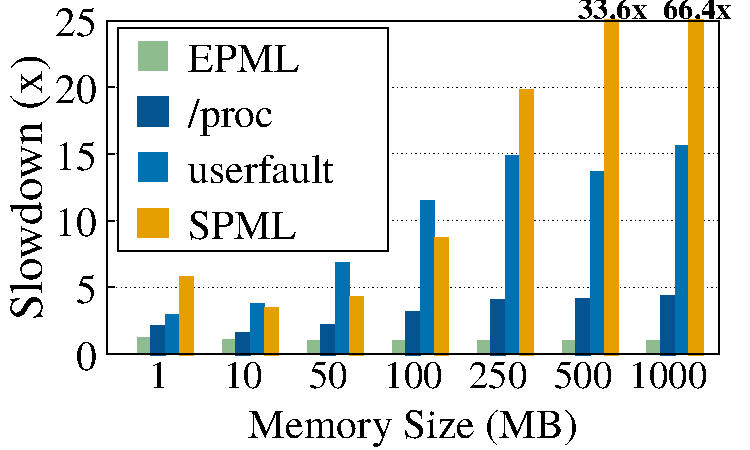
\includegraphics[width=\linewidth]{fig/slowdown}%
}		
		\captionof{figure}{\small Overhead of each tracking technique on the micro-benchmark.}
		\label{fig:microbench-overheads}
	\end{minipage}
	\vspace*{.1cm}
\end{figure}				
			\end{block}
        \end{frame}        
%%%%%%%%%%%%%%%%%%%%%%%%%%%%%%%%%%%%%%%%%%%%%%%%%%%%%%%%%%%%%%%%%%%%%%%%%%%%%%%%%%%
        \begin{frame}
                \frametitle{Evaluations}
				\begin{block}{Impact on Boehm}
\begin{figure}[!h]
	\centering 
	%\vspace*{-.2cm}
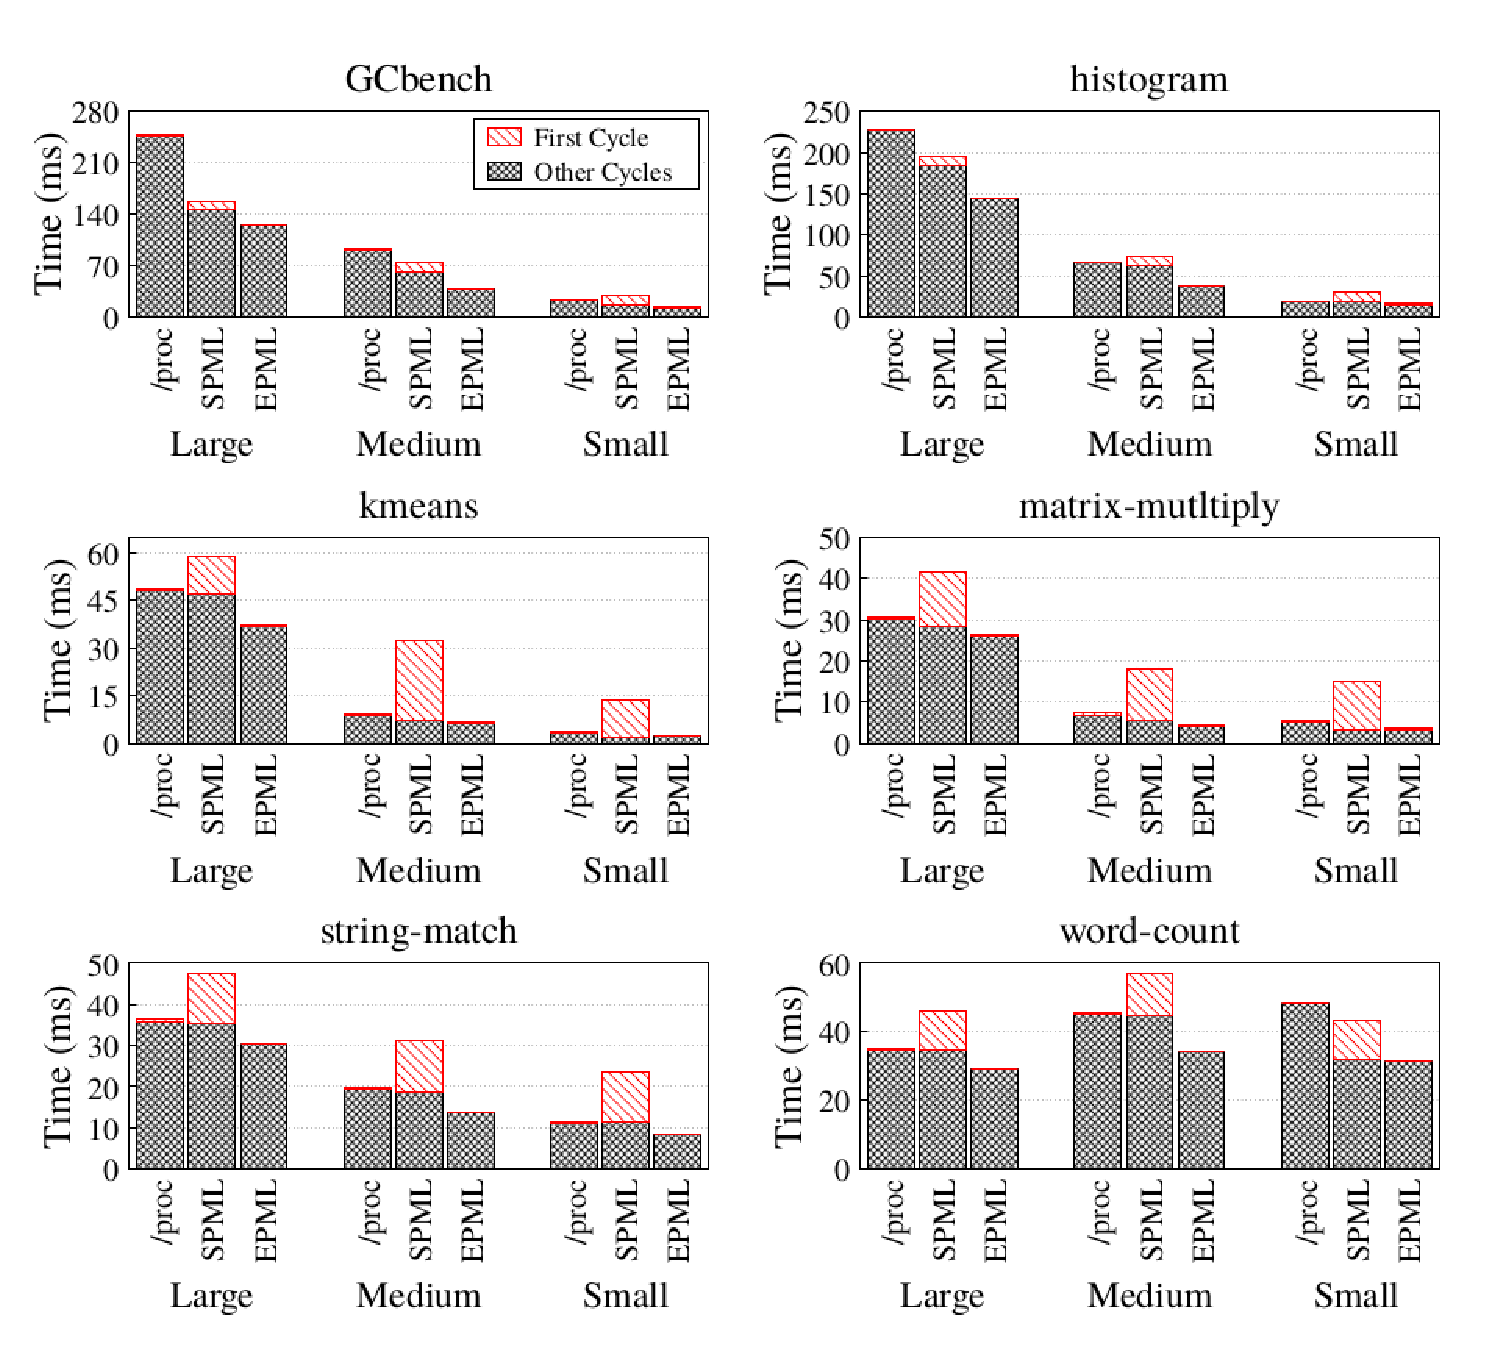
\includegraphics[width=.45\linewidth]{fig/boehm-results-tracker}

%		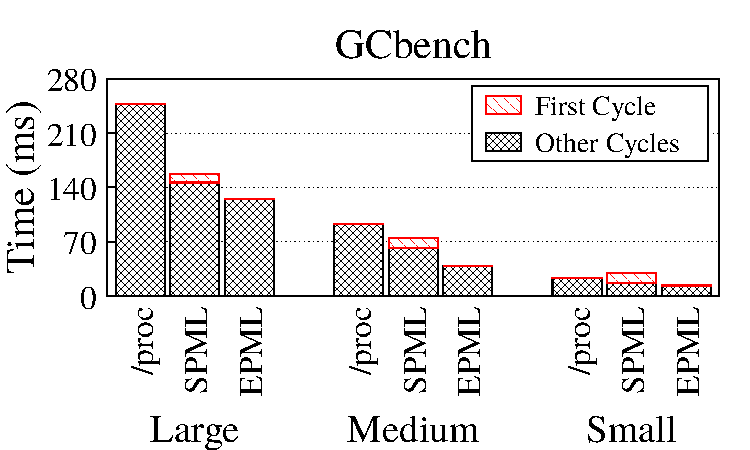
\includegraphics[width=.2\linewidth]{fig/gcbench_stacked}
%		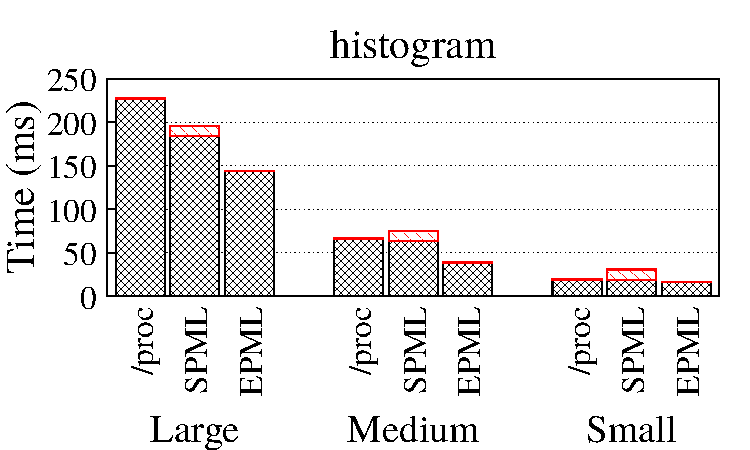
\includegraphics[width=.2\linewidth]{fig/histogram_stacked}
%		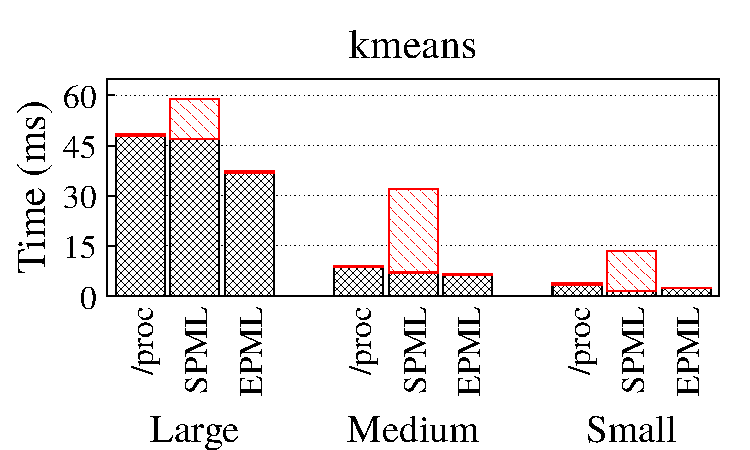
\includegraphics[width=.2\linewidth]{fig/kmeans_stacked}
%		
%		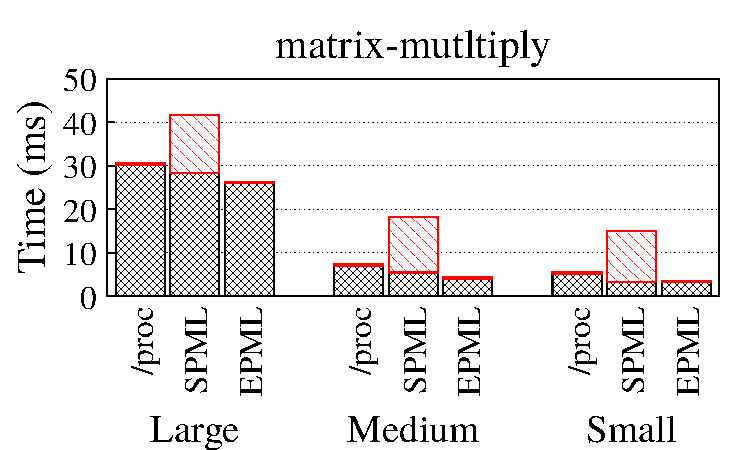
\includegraphics[width=.2\linewidth]{fig/matrix-mul_stacked}
%		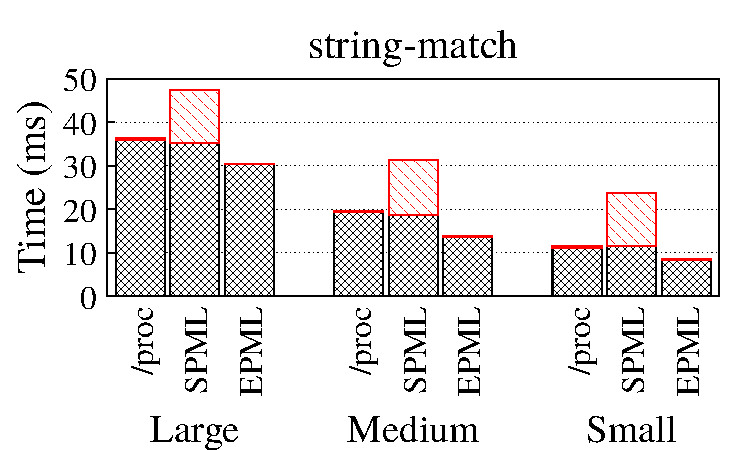
\includegraphics[width=.2\linewidth]{fig/string-match_stacked}
%		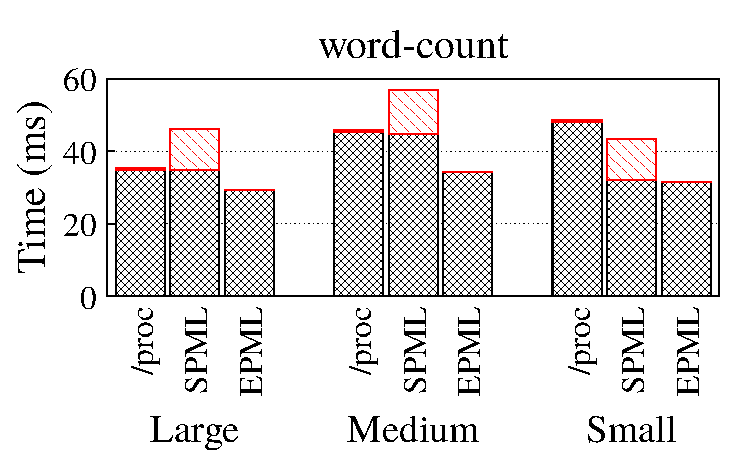
\includegraphics[width=.2\linewidth]{fig/word-count_stacked}
		
	\caption{\scriptsize We highlight the first GC cycle during which Boehm performs reverse mapping with SPML.}
	\label{fig:boehm-results-tracker}
\end{figure}											
			\end{block}
        \end{frame}
%%%%%%%%%%%%%%%%%%%%%%%%%%%%%%%%%%%%%%%%%%%%%%%%%%%%%%%%%%%%%%%%%%%%%%%%%%%%%%%%%%%
        \begin{frame}
                \frametitle{Evaluations}
				\begin{block}{Impact on applications}
\begin{figure}[!htp]
	\centering 
\fcolorbox{white}{white}{					
		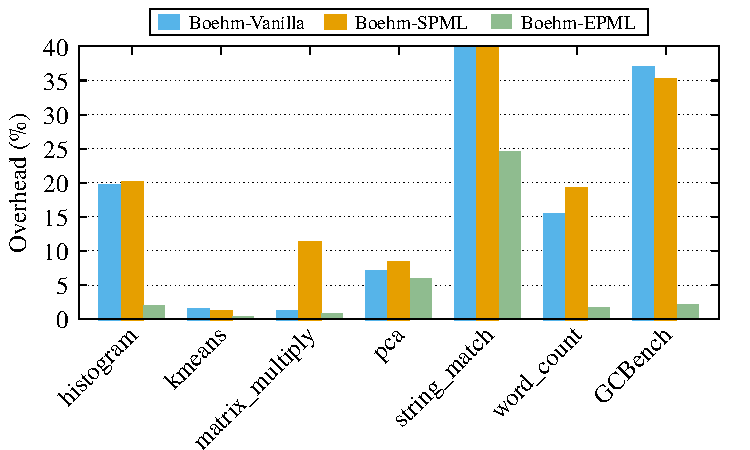
\includegraphics[width=.32\linewidth]{fig/tracked_large}
		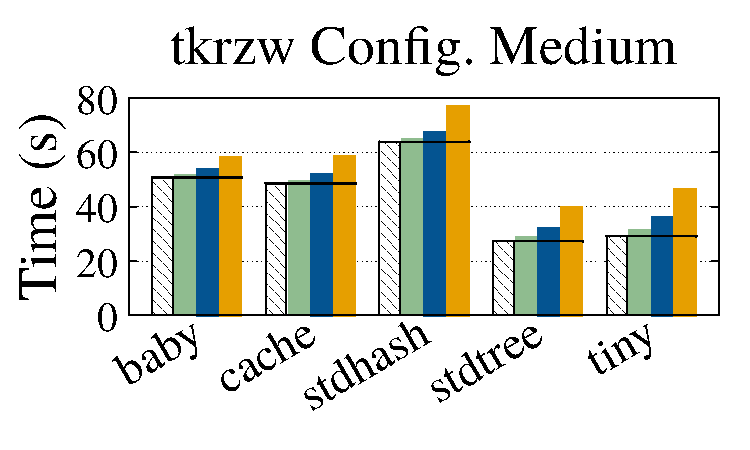
\includegraphics[width=.32\linewidth]{fig/tracked_medium}
		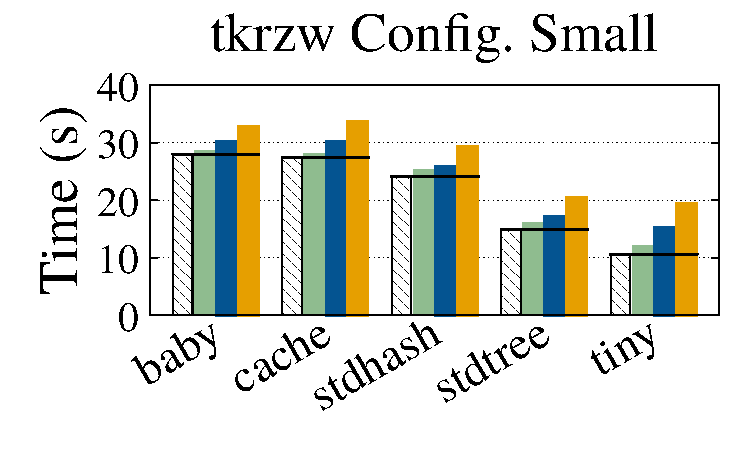
\includegraphics[width=.32\linewidth]{fig/tracked_small}
}		
	\caption{\small Impact of Boehm GC.}
	\label{fig:boehm-results-tracked}
\end{figure}											
			\end{block}
        \end{frame}      
%%%%%%%%%%%%%%%%%%%%%%%%%%%%%%%%%%%%%%%%%%%%%%%%%%%%%%%%%%%%%%%%%%%%%%%%%%%%%%%%%%%
        \begin{frame}
                \frametitle{Evaluations}
				\begin{block}{Impact on CRIU}
\begin{figure}[!htp]
	\centering 
	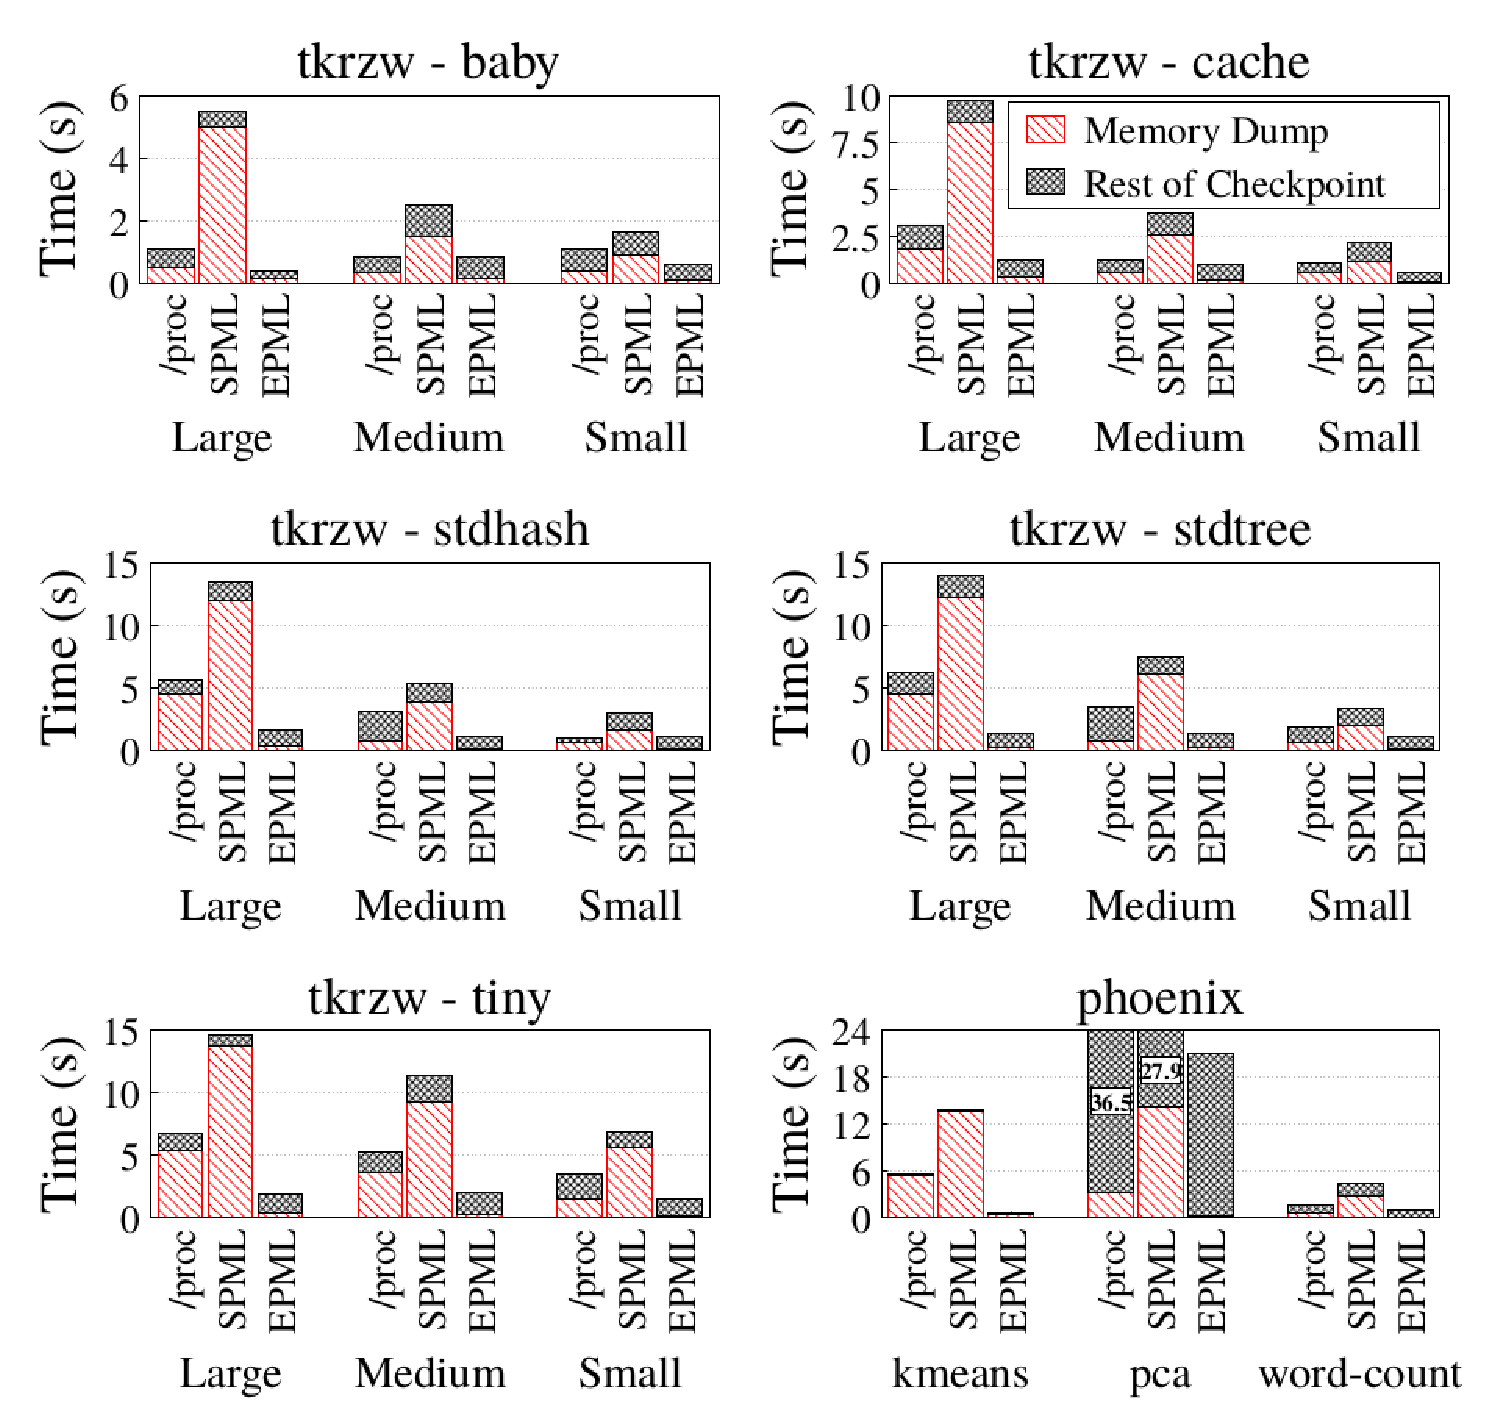
\includegraphics[width=.45\linewidth]{fig/criu-results-tracker}
%	\begin{subfigure}[b]{\columnwidth}
%		\centering
%\fcolorbox{white}{white}{							
%		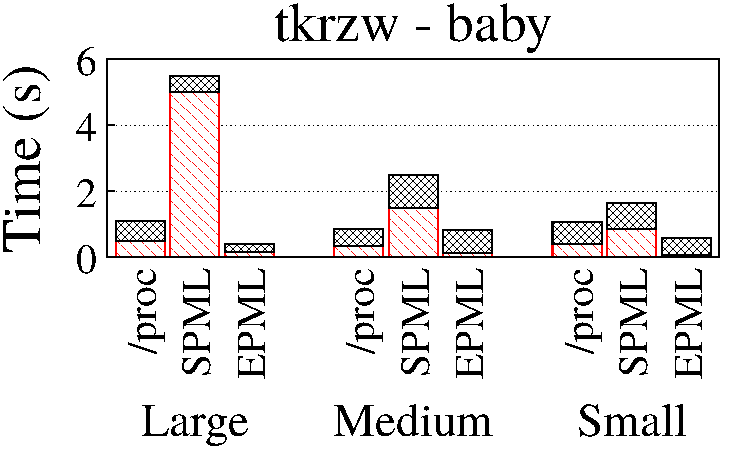
\includegraphics[width=.48\linewidth]{fig/baby_stacked}
%		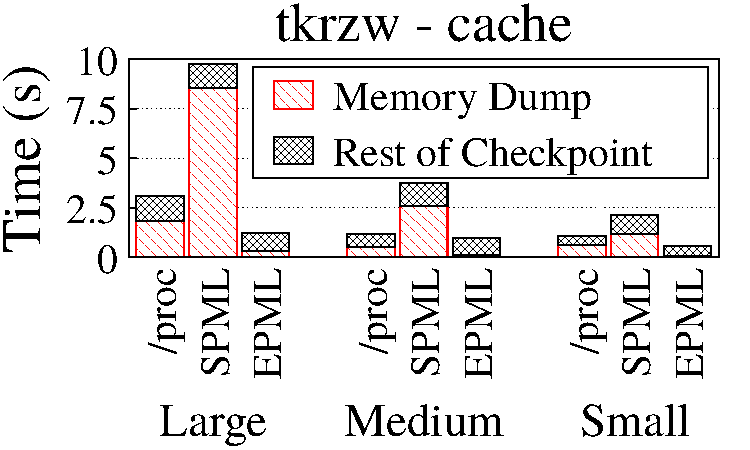
\includegraphics[width=.48\linewidth]{fig/cache_stacked}
%}		
%		\vspace{.3cm}
%	\end{subfigure} 
%	\begin{subfigure}[b]{\columnwidth}
%\fcolorbox{white}{white}{								
%		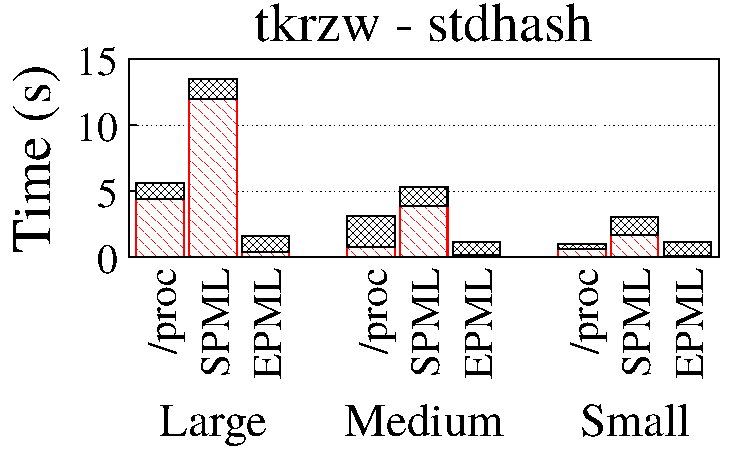
\includegraphics[width=.48\linewidth]{fig/stdhash_stacked}
%		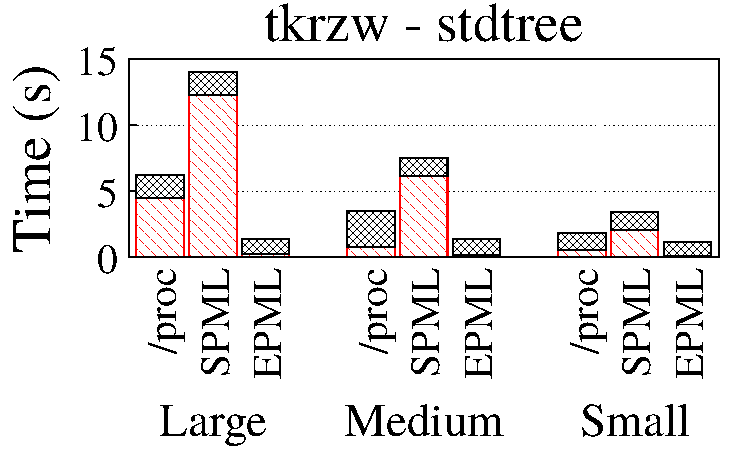
\includegraphics[width=.48\linewidth]{fig/stdtree_stacked}
%}		
%		\vspace{.3cm}
%	\end{subfigure} 
%	\begin{subfigure}[b]{\columnwidth}
%\fcolorbox{white}{white}{							
%		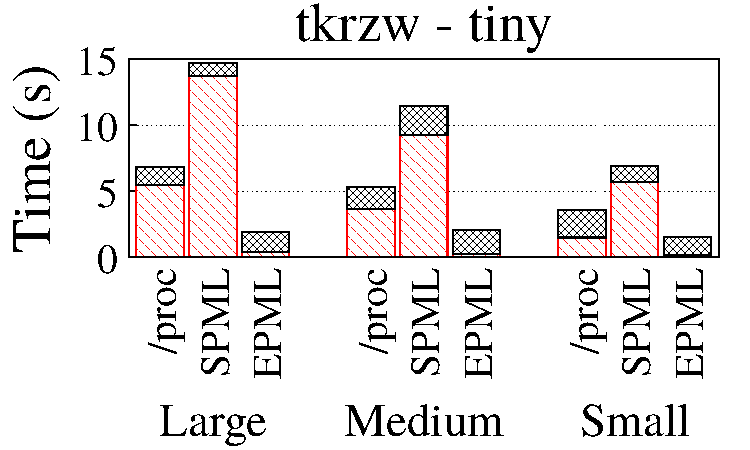
\includegraphics[width=.48\linewidth]{fig/tiny_stacked}
%		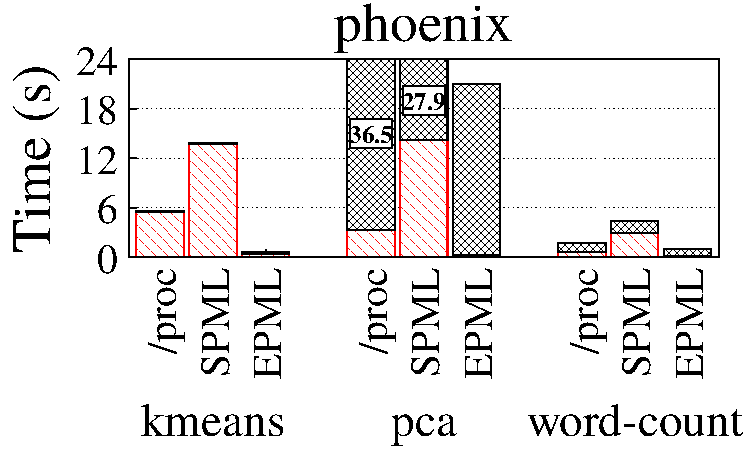
\includegraphics[width=.48\linewidth]{fig/phoenix_stacked}
%}		
%	\end{subfigure} 
	\caption{\scriptsize We highlight MD phase during which CRIU performs reverse mapping with SPML.}
	\label{fig:criu-results-tracker}
\end{figure}											
			\end{block}
        \end{frame}        
%%%%%%%%%%%%%%%%%%%%%%%%%%%%%%%%%%%%%%%%%%%%%%%%%%%%%%%%%%%%%%%%%%%%%%%%%%%%%%%%%%%
        \begin{frame}
                \frametitle{Evaluations}
				\begin{block}{Impact on the checkpointed app}
\begin{figure}[!h]
	\centering 
	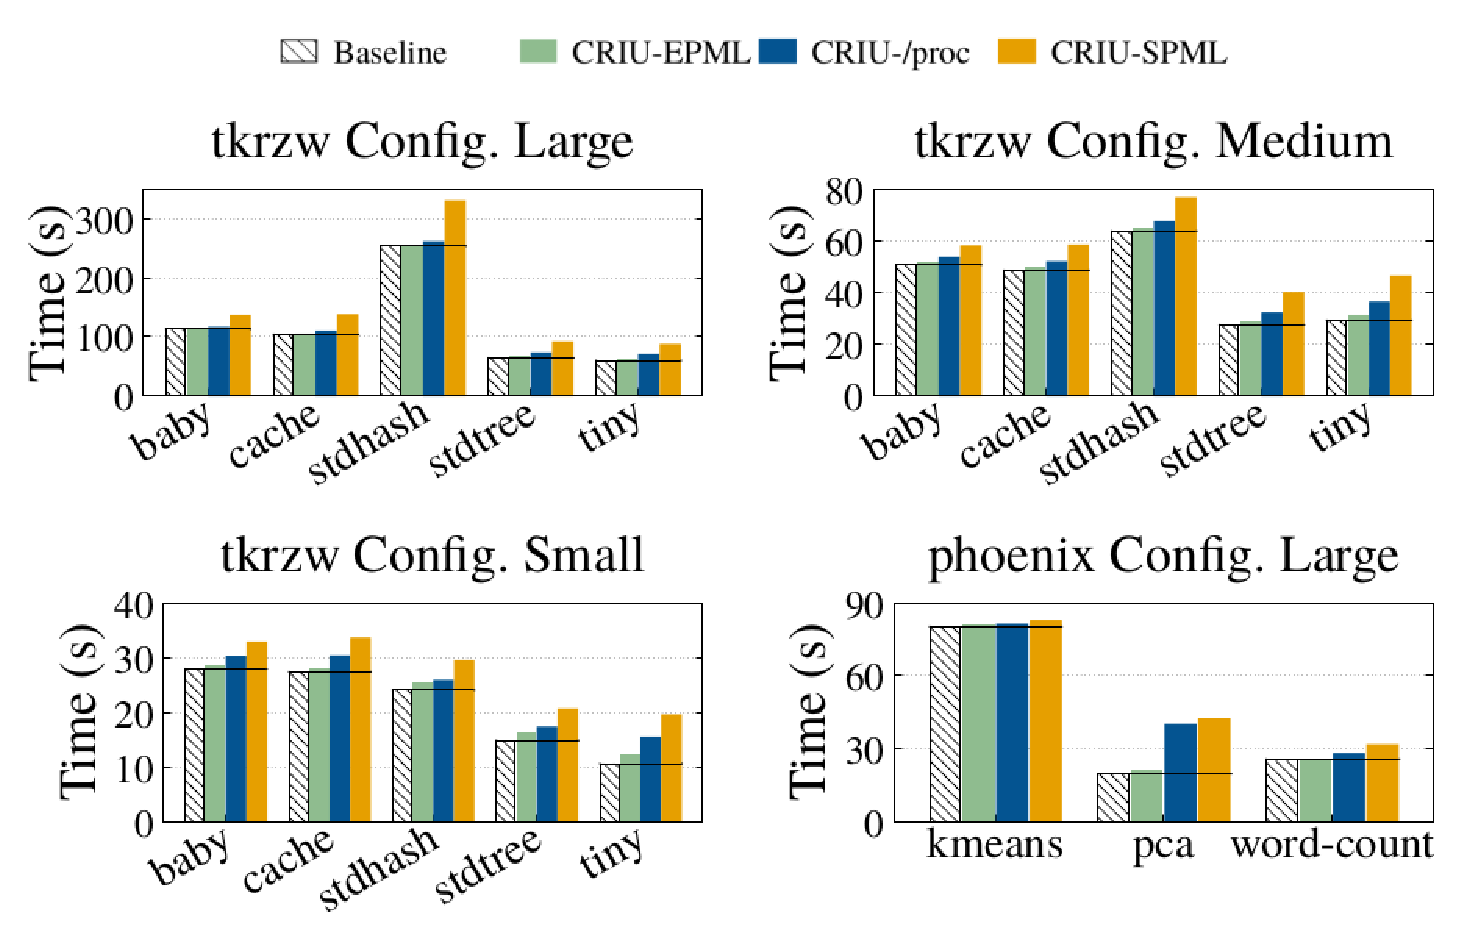
\includegraphics[width=.6\linewidth]{fig/criu-results-tracked}
%	\begin{subfigure}[b]{\columnwidth}
%		\centering
%		\hspace{.15cm}
%\fcolorbox{white}{white}{									
%		
\includegraphics[scale=.15]{fig/legend_tracked}
%}		
%		\vspace{.15cm}
%	\end{subfigure}
%	\begin{subfigure}[b]{\columnwidth}
%		\centering 
%\fcolorbox{white}{white}{									
%		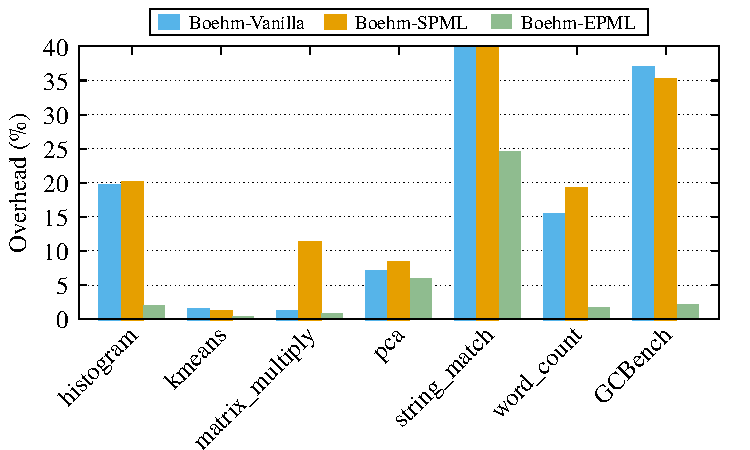
\includegraphics[width=.48\linewidth]{fig/tracked_large}
%		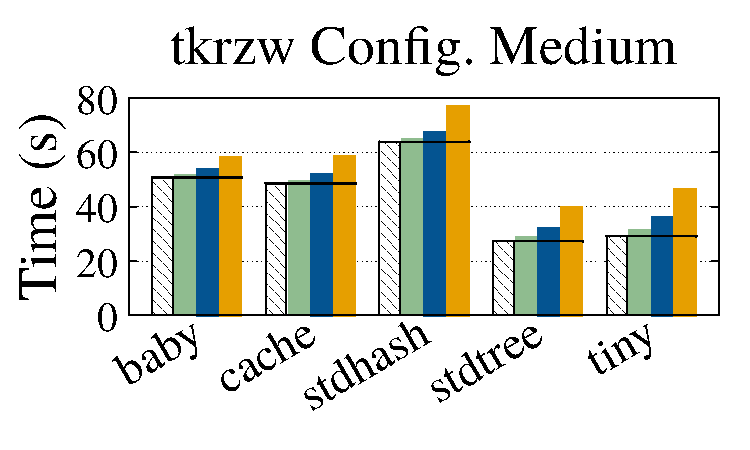
\includegraphics[width=.48\linewidth]{fig/tracked_medium}
%		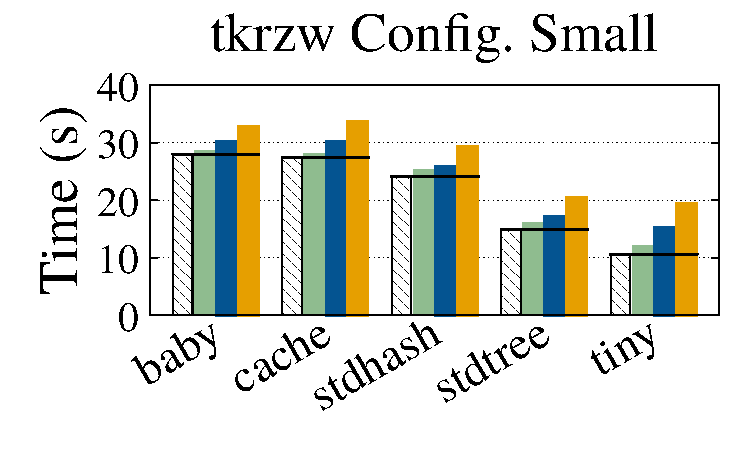
\includegraphics[width=.48\linewidth]{fig/tracked_small}
%		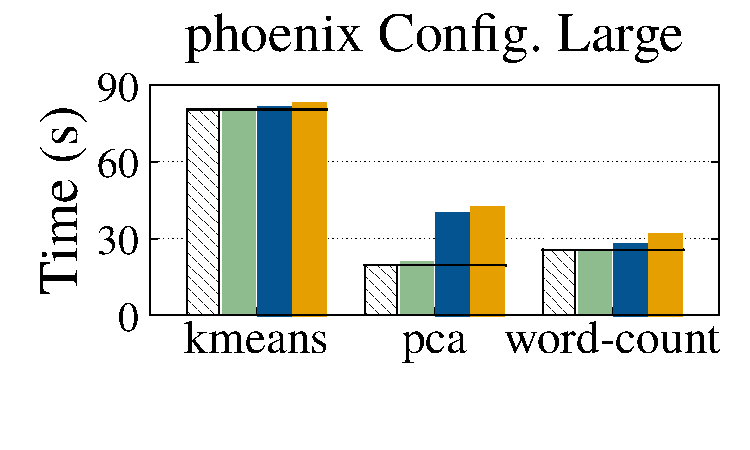
\includegraphics[width=.48\linewidth]{fig/tracked_phoenix}
%}		
%	\end{subfigure}
%	\caption{Impact of CRIU on Tracked execution time when using \texttt{/proc}, SPML and EPML techniques.}
%	\label{fig:criu-results-tracked}
%	\vspace*{.2cm}
\end{figure}										
			\end{block}
        \end{frame}         
%%%%%%%%%%%%%%%%%%%%%%%%%%%%%%%%%%%%%%%%%%%%%%%%%%%%%%%%%%%%%%%%%%%%%%%%%%%%%%%%%%%
        \begin{frame}
                \frametitle{Evaluations}
				\begin{block}{Summary}
					\begin{itemize}
						\item Impact on the tracker
						\begin{itemize}
							\item SPML induces up to 5$\times$ slowdown on CRIU and 3$\times$ slowdown on Boehm GC.
							\item EPML brings up to 4$\times$ speedup compared to \texttt{/proc} and 13$\times$ speedup compared to SPML for CRIU; up to 2$\times$ speedup compared to \texttt{/proc} and up to 6$\times$ speedup compared to SPML.
						\end{itemize}																							
					\end{itemize}
			\end{block}
        \end{frame}  
%%%%%%%%%%%%%%%%%%%%%%%%%%%%%%%%%%%%%%%%%%%%%%%%%%%%%%%%%%%%%%%%%%%%%%%%%%%%%%%%%%%
        \begin{frame}
                \frametitle{Evaluations}
				\begin{block}{Summary}
					\begin{itemize}		
						\item Impact on the application performance
						\begin{itemize}
							\item \texttt{/proc}, which is the default solution implemented in both CRIU and Boehm, incurs an overhead of up to 102\% with CRIU on the Phoenix \texttt{pca} application, and up to 232\% with Boehm on the Phoenix \texttt{string-match} application.
							\item The overhead of SPML is up to 114\% with CRIU and 273\% with Boehm on the same applications.
							\item EPML leads to the lowest overhead, which is about 7\% with CRIU and 24\% with Boehm.
						\end{itemize}																							
					\end{itemize}
			\end{block}
        \end{frame}           
%%%%%%%%%%%%%%%%%%%%%%%%%%%%%%%%%%%%%%%%%%%%%%%%%%%%%%%%%%%%%%%%%%%%%%%%%%%%%%%%%%%
        \begin{frame}
        \frametitle{In this talk} 
			\begin{block}{OoH for Intel SPP}
				\begin{itemize}
					\item for reducing memory overhead of guard page-based secured heap memory allocators
					\item work in progress
				\end{itemize}
			\end{block}
			\begin{block}{OoH for Intel PML}
				\begin{itemize}
					\item for improving process/container checkpointing, concurrent GCs
					\item excellent results
				\end{itemize}
			\end{block}	
			\begin{block}{The main message}
				\begin{itemize}
					\item When thinking hypervisor-oriented hardware virtualization features, please think how they can be also used by processes from inside VMs, this may need few efforts
				\end{itemize}
			\end{block}							
        \end{frame}                       
%%%%%%%%%%%%%%%%%%%%%%%%%%%%%%%%%%%%%%%%%%%%%%%%%%%%%%%%%%%%%%%%%%%%%%%%%%%%%%
\begin{frame}
	\frametitle{For questions}
	\begin{itemize}
		\item Stella Bitchebe
		\begin{itemize}
			\item mail: celestine-stella.ndonga-bitchebe@ens-lyon.fr
			\item Phone: 00 33 6 54 63 42 74
			\item Address: 3 Rue du Kiwi, Lyon.
		\end{itemize}
		\item Yves Kone
		\begin{itemize}
			\item mail: yves.kone@ens-lyon.fr
			\item Phone: 00 33 6 55 65 45 75
			\item Address: 3 Avenue du buffle, Lyon.
		\end{itemize}		
	\end{itemize}
\end{frame}
%%%%%%%%%%%%%%%%%%%%%%%%%%%%%%%%%%%%%%%%%%%%%%%%%%%%%%%%%%%%%%%%%%%%%%%%%%%%%%
%%%%%%%%%%%%%%%%%%%%%%%%%%%%%%%%%%%%%%%%%%%%%%%%%%%%%%%%%%%%%%%%%%%%%%%%%%%%%%%%
      
\end{document}
